\chapter{Experimental results}
    This chapter will discuss the experimental setting used and the results of the trained models.
\section{Experimental Setting}
    The model as well as the hyperparamters are defined using Tensorflow and Keras. 
    The model was trained for single region segmentation as well as multi-region segmentation where all 14 regions were predicted all at once.
    The hyperparemeter set up was slightly different for training a model for a single region vs multiple regions. 
    For the single region training the learning rate was 1e-5 and the batch size was 32 for U-net and 3 for the dilation models. 
    The batch size varied depending on the model as the dilation models needed more memory.  
    The models in the single region were trained for at least 128 epochs in order to ensure that the model was trained sufficiently, but not over fitting the data. 
    
    For multiple region training the learning used was 2e-5 and the batch size was 32 for U-net and the U-net dilation and 16 for the modified dilation VGG-16 models. 
    The learning rate is larger because since there was much more to learn the models struggled in the beginning to learn well.
    The multiple region models were trained for much longer than the single region training and needed to be trained for at least 300 epochs in order to train the model sufficiently.
    The multiple region models learning rate was changed because the training for those models were much slower and so utilizing a higher learning rate make the learning much faster.
    Each model is trained using the ADAM optimizer as described in ~\cite{Kingma2014AdamAM}. 
    The input images were also shuffled randomly in order to decrease the bias that the model might learn. 
    The experiments were trained on a 10GB NVIDIA GTX 1080 Ti. 
    
\subsection{Image Data}
    As explained before a total of 40 rats were imaged with a total of 120 MRI images taken. 
    Due to some problems with imaging only 115 animal scans were available for use within the model. 
    The data was split between a training set, a validation set, and test set. 
    Since the data is also split between 4 different animal groups the validation and test dataset has one animal from each group to see how each group performs from the model. 
   Each animal has MR images at three different time points as well and so the validation/test sets consist of 12 different animal MR images while the training dataset consists of 103 animal MR images. 
    Data augmentation was also utilized as explained before and the dataset was doubled and data augmentation applied to the replicated data. 
    The training dataset consists of a total of 206 MR images each of size 128x128x44 or 9,064 total 2D 1MR images while the validation and test sets consists of 12 MR images each of size 128x128xx44 or 528 2D MR images. 

\section{Visualization of segmentation results for single region}
    For the single segmentation, the segmentation chosen was for the medial thalamus. 
    This region was chosen because it was the smallest region as well as a region that changed throughout the groups.
    

\subsection{Models}
    This section is dedicated to show the different models tested and to compare them for single region segmentation of the MR images. 
    This is very challenging because the regions are so small within the 128x128x44 MRI images that the model needs to take that into account. 
    Table `\ref{tab.single_model_results} shows the results for the average dice score coefficient for single region segmentation.
    U-net gave the most consistent answers and was the easiest to implement while there were some problems when training the dilation VGG-16 model.
    U-net performs much better than dilation VGG-16 in the training data but not much better according to the validation data and we see they are quite close with u-net only slightly outperforming dilation VGG-16. 
    Let us take a closer look at each model.
    
\begin{table}[tbh]
% increase table row spacing, adjust to taste
\renewcommand{\arraystretch}{1}
% if using array.sty, it might be a good idea to tweak the value of
% \extrarowheight as needed to properly center the text within the cells
\centering
% Some packages, such as MDW tools, offer better commands for making tables
% than the plain LaTeX2e tabular which is used here.
\begin{tabular}{|c|c|c|}
\hline
\textbf{Model} & \textbf{training DSC} & \textbf{validation DSC}\\
\hline
U-net & 0.997 & 0.811\\ %weights_singleLabel1_dilation_2_300.h5     
%#\hline
%dilation layer & 0.0000\\%weights_singleLabel1_reduceModel_1_128.h5
\hline
dilation VGG-16 & 0.698 & 0.801\\ %weights_singleLabel1_1_128.h5 
\hline
\end{tabular}
\caption{DSC scores comparing U-net and the dilation VGG-16 models}
\label{tab.single_model_results}
\end{table}


\subsubsection{U-net}
    Here are the training results for single region u-net as discussed before. 
    Figure ~\ref{fig:results_single_unet_train} shows the training and validation results of the model. 
    U-net was able to learn the training dataset very well with a training DSC of 0.99 while the validation dataset leaned quite well at 0.803.
    After the 50 epoch the model DSC didn't go up much at all and stabilized while the training DSC slowly increased.
    Table ~\ref{tab.single_model_results_Unet} shows the overall results for the model. 
    The control group or VEH results aren't available for this calculation.
    What is interesting is that the model performs the best on the D28 images for DFP and MDZ. 
    The D28 images especially for DFP are the most inconsistent because of brain cell death from seizures, while the D03 images are the most consistent as they are the closest to a healthy rat brain. 
    This is also shown in the variation among the DSC of the D03 data compared to the D28 data, where the D03 data is more consistent than the D28 data. 
    
    
\begin{figure}[tbh]
\centering
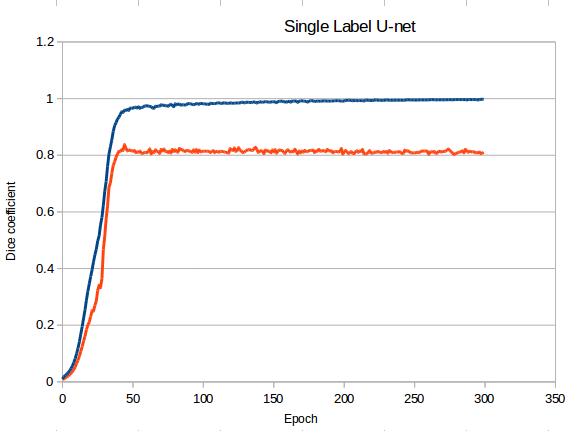
\includegraphics[width=\textwidth]{results/train_results_single_unet.png}
% where an .eps filename suffix will be assumed under latex,
% and a .pdf suffix will be assumed for pdflatex
\caption{Training the U-net model. Blue curve is training curve and the red curve is the validation curve. }
\label{fig:results_single_unet_train}
\end{figure}

\begin{table}[tbh]
% increase table row spacing, adjust to taste
\renewcommand{\arraystretch}{1}
% if using array.sty, it might be a good idea to tweak the value of
% \extrarowheight as needed to properly center the text within the cells
\centering
% Some packages, such as MDW tools, offer better commands for making tables
% than the plain LaTeX2e tabular which is used here.
\begin{tabular}{|c|c|c|c|}
\hline
\textbf{Group} & \textbf{D03}& \textbf{D07}& \textbf{D28}\\
\hline
DFP & 0.755 & 0.836 & 0.872\\      
\hline
DZP & 0.765 & 0.814 & 0.788\\
\hline
MDZ & 0.821 & 0.769 & 0.832\\ 
\hline
\end{tabular}
\caption{DSC scores of test data for single model U-net}
\label{tab.single_model_results_Unet}
\end{table}


    Figure ~\ref{fig:results_single_unet_DFP} shows the results when applied to the DFP test images. 
    If we compare the different days the biggest difference are the D28 images compared to the D03 and D07 images. 
    The medial thalamus shifted as brain changed due to the seizures. 
    The brighter regions or the ventricles also increased significantly compared to in the beginning. 
    When just looking at the results it seems they match up quite well with the ground truth with some minor differences. 
    Figure ~\ref{fig:results_single_unet_DZP} and figure ~\ref{fig:results_single_unet_MDZ} show the results for the DZP and the MDZ test images, relatively.
    If we compare the DZP and MDZ images with the DFP images the ventricles in the DZP and MDZ are much smaller and the general shape of the brain hasn't changed as significantly as the DFP animals.
    One interesting thing to note is that in figure ~\ref{fig:results_single_unet_MDZ} the day 28 image has a ground truth but no prediction. 
    This is interesting because it shows that the model has to learn to segment the regions that are on different slice numbers or grouped with different regions. 
    This is were the convolutional layers come into play as they make the model spatially invariant and so no matter which slice the region is at as long as the characteristics are consistent the model will still predict a region. 
    Upon further inspection D28 slice 23 in the MDZ animals is the start of the medial thalamus and in the images where the medial thalamus starts with a very small region like in the MDZ animal case we don't get a prediction. 
    Overall the U-net preforms quite well on the single region segmentation with only some slight differences in the predictions. 
    We will explain later why these slight differences are acceptable. 
    

\begin{figure}[!ht]  
   \centering % <-- added
\begin{subfigure}{0.35\textwidth}
  \includegraphics[width=\linewidth]{results/single_unet/"DFP01 R14-189-D03_23".png}
  \caption{D03 slice 23}
\end{subfigure}\hfil % <-- added
\begin{subfigure}{0.35\textwidth}
  \includegraphics[width=\linewidth]{results/single_unet/"DFP01 R14-189-D03_25".png}
  \caption{D03 slice 25}
\end{subfigure}

\medskip
\begin{subfigure}{0.35\textwidth}
  \includegraphics[width=\linewidth]{results/single_unet/"DFP01 R14-189-D07_23".png}
  \caption{D07 slice 23}
\end{subfigure}\hfil % <-- added
\begin{subfigure}{0.35\textwidth}
  \includegraphics[width=\linewidth]{results/single_unet/"DFP01 R14-189-D07_25".png}
  \caption{D07 slice 25}
\end{subfigure}

\medskip
\begin{subfigure}{0.35\textwidth}
  \includegraphics[width=\linewidth]{results/single_unet/"DFP01 R14-189-D28_23".png}
  \caption{D28 slice 23}
\end{subfigure}\hfil % <-- added
\begin{subfigure}{0.35\textwidth}
  \includegraphics[width=\linewidth]{results/single_unet/"DFP01 R14-189-D28_25".png}
  \caption{D28 slice 25}
\end{subfigure}
  
  \caption{Results for DFP animal group at day 3, day 7, day 28 on single region U-net. The red region is the predicted output the model sent and the blue region is the ground truth.}
  \label{fig:results_single_unet_DFP}
\end{figure}


\begin{figure}[!htb]  
\centering % <-- added
\begin{subfigure}{0.35\textwidth}
  \includegraphics[width=\linewidth]{results/single_unet/"DZP01 R14-187-D03_23".png}
  \caption{D03 slice 23}
\end{subfigure}\hfil
\begin{subfigure}{0.35\textwidth}
  \includegraphics[width=\linewidth]{results/single_unet/"DZP01 R14-187-D03_25".png}
  \caption{D03 slice 25}
\end{subfigure}

\medskip
\begin{subfigure}{0.35\textwidth}
  \includegraphics[width=\linewidth]{results/single_unet/"DZP01 R14-187-D07_23".png}
  \caption{D07 slice 23}
\end{subfigure}\hfil
\begin{subfigure}{0.35\textwidth}
  \includegraphics[width=\linewidth]{results/single_unet/"DZP01 R14-187-D07_25".png}
  \caption{D07 slice 25}
\end{subfigure}

\medskip
\begin{subfigure}{0.35\textwidth}
  \includegraphics[width=\linewidth]{results/single_unet/"DZP01 R14-187-D28_23".png}
  \caption{D28 slice 23}
\end{subfigure}\hfil
\begin{subfigure}{0.35\textwidth}
  \includegraphics[width=\linewidth]{results/single_unet/"DZP01 R14-187-D28_25".png}
  \caption{D28 slice 25}
\end{subfigure}
  
  \caption{Results for DZP animal group at day 3, day 7, day 28 on single region U-net. The red region is the predicted output the model sent and the blue region is the ground truth.}
  \label{fig:results_single_unet_DZP}
\end{figure}



\begin{figure}[!htb]  
   \centering % <-- added
\begin{subfigure}{0.35\textwidth}
  \includegraphics[width=\linewidth]{results/single_unet/"MDZ01 R14-190-D03_23".png}
  \caption{D03 slice 23}
\end{subfigure}\hfil % <-- added
\begin{subfigure}{0.35\textwidth}
  \includegraphics[width=\linewidth]{results/single_unet/"MDZ01 R14-190-D03_25".png}
  \caption{D03 slice 25}
\end{subfigure}

\medskip
\begin{subfigure}{0.35\textwidth}
  \includegraphics[width=\linewidth]{results/single_unet/"MDZ01 R14-190-D07_23".png}
  \caption{D07 slice 23}
\end{subfigure}\hfil % <-- added
\begin{subfigure}{0.35\textwidth}
  \includegraphics[width=\linewidth]{results/single_unet/"MDZ01 R14-190-D07_25".png}
  \caption{D07 slice 25}
\end{subfigure}

\medskip
\begin{subfigure}{0.35\textwidth}
  \includegraphics[width=\linewidth]{results/single_unet/"MDZ01 R14-190-D28_23".png}
  \caption{D28 slice 23}
\end{subfigure}\hfil % <-- added
\begin{subfigure}{0.35\textwidth}
  \includegraphics[width=\linewidth]{results/single_unet/"MDZ01 R14-190-D28_25".png}
  \caption{D28 slice 25}
\end{subfigure}
  
  \caption{Results for MDZ animal group at day 3, day 7, day 28 on single region U-net. The red region is the predicted output the model sent and the blue region is the ground truth. }
  \label{fig:results_single_unet_MDZ}
\end{figure}

\subsubsection{Dilation VGG-16}
    Here are the training results for the modified dilation VGG-16 model. 
    Figure ~\ref{fig:results_single_dilation_train} shows the training and validation results. 
    It is interesting to note how the validation DSC is larger than the training DSC.
    This can be attributed to the fact that the validation data is less complex than the training data due to the data augmentation. 
    The dilation VGG-16 model also has much less parameters than U-net and so the model can't learn the more complex training data as well as the validation data. 
    Another interesting thing to note is that the training and validation curves shoot up from the 1st epoch and mainly stabilize at the epoch 20. 
    Table ~\ref{tab.single_model_results_dilation} shows the results of the dilation VGG-16 model on the test data. Compared to U-net the DSC values are much lower for the dilation VGG-16 model. 
    This means that the dilation VGG-16 model doesn't generalize as well as the U-net model. 
    This could be attributed to the parameters of the model or how its structured is not ideal for the single segmentation task. 
    The D03 DSC's in the table are on average a higher DSC compared to D07 and D28 and the variation is smaller. 
    D28 DSC's the average is the least and variation the largest.
    This is because D28 has the most variation so the dilation VGG-16 model became slightly biased to segment the earlier times better since they are more consistent.
    In the case of U-net, it had enough parameters to still be able to learn the D28 dataset as well. 

\begin{figure}[!tbh]
\centering
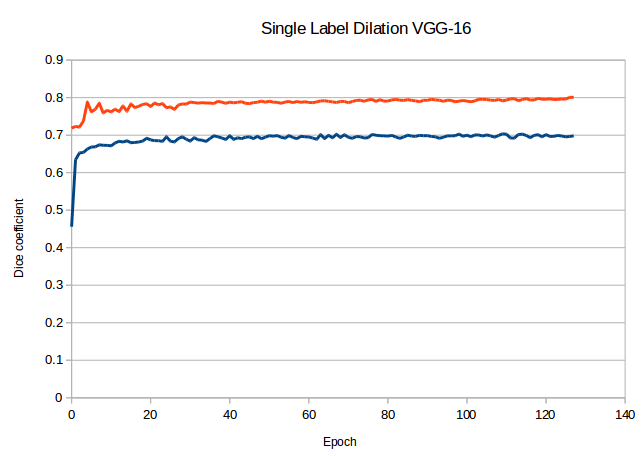
\includegraphics[width=\textwidth]{results/train_results_single_dilation.png}
% where an .eps filename suffix will be assumed under latex,
% and a .pdf suffix will be assumed for pdflatex
\caption{Training the dilation VGG-16 model. Blue curve is training curve and the red curve is the validation curve. }
\label{fig:results_single_dilation_train}
\end{figure}

\begin{table}[tbh]
% increase table row spacing, adjust to taste
\renewcommand{\arraystretch}{1}
% if using array.sty, it might be a good idea to tweak the value of
% \extrarowheight as needed to properly center the text within the cells
\centering
% Some packages, such as MDW tools, offer better commands for making tables
% than the plain LaTeX2e tabular which is used here.
\begin{tabular}{|c|c|c|c|}
\hline
\textbf{Group} & \textbf{D03}& \textbf{D07}& \textbf{D28}\\
\hline
DFP & 0.711 & 0.551 & 0.706\\      
\hline
DZP & 0.729 & 0.681 & 0.563\\
\hline
MDZ & 0.665 & 0.650 & 0.617\\ 
\hline
VEH & 0.649 & 0.675 & 0.635\\ 
\hline
\end{tabular}
\caption{DSC scores of test data for single model dilation VGG-16}
\label{tab.single_model_results_dilation}
\end{table}


Figure ~\ref{fig:results_single_dilation_DFP}, ~\ref{fig:results_single_dilation_DZP}, ~\ref{fig:results_single_dilation_MDZ}, and ~\ref{fig:results_single_dilation_VEH} show the segmentation images of the dilation VGG-16 model applied to the test image. 
Compared to the U-net results the dilation VGG-16 predictions are more circular. 
This causes the regions to match horizontally, but vertically the prediction overshoots the ground truth and lowers the overall DSC.
This is the reason why the DSC for the dilation VGG-16 model performs much lower than U-net.
One difference is that for figure ~\ref{fig:results_single_dilation_MDZ}, MDZ D28 slice 23 the dilation VGG-16 model was able to predict a region though larger than the ground truth where U-net didn't predict a region here. 
Another interesting thing to note is in figure ~\ref{fig:results_single_dilation_DZP} in D28 slice 23 that dilation VGG-16 model predicted the medial thalamus even though there is no ground truth.
This could be attributed to the modified dilation VGG-16 model not learning about the results as well as u-net.
In figure ~\ref{fig:results_single_dilation_DFP} the D07 segmentation got the worst results at a DSC of 0.55 and in slice 23 their is no prediction. 
This is interesting as it seems like the predictions for D07 and D28 are very similar, which causes a better performance for D28 and a worse one for D07.

\begin{figure}[!htb]  
    \centering % <-- added
\begin{subfigure}{0.35\textwidth}
  \includegraphics[width=\linewidth]{results/single_dilation/"DFP01 R14-189-D03_23".png}
  \caption{D03 slice 23}
\end{subfigure}\hfil % <-- added
\begin{subfigure}{0.35\textwidth}
  \includegraphics[width=\linewidth]{results/single_dilation/"DFP01 R14-189-D03_25".png}
  \caption{D03 slice 25}
\end{subfigure}

\medskip
\begin{subfigure}{0.35\textwidth}
  \includegraphics[width=\linewidth]{results/single_dilation/"DFP01 R14-189-D07_23".png}
  \caption{D07 slice 23}
\end{subfigure}\hfil % <-- added
\begin{subfigure}{0.35\textwidth}
  \includegraphics[width=\linewidth]{results/single_dilation/"DFP01 R14-189-D07_25".png}
  \caption{D07 slice 25}
\end{subfigure}

\medskip
\begin{subfigure}{0.35\textwidth}
  \includegraphics[width=\linewidth]{results/single_dilation/"DFP01 R14-189-D28_23".png}
  \caption{D28 slice 23}
\end{subfigure}\hfil % <-- added
\begin{subfigure}{0.35\textwidth}
  \includegraphics[width=\linewidth]{results/single_dilation/"DFP01 R14-189-D28_25".png}
  \caption{D28 slice 25}
\end{subfigure}
  
  \caption{Results for DFP animal group at day 3, day 7, day 28 on single region dilation VGG-16. The red region is the predicted output the model sent and the blue region is the ground truth.}
  \label{fig:results_single_dilation_DFP}
\end{figure}


\begin{figure}[!htb]  
    \centering % <-- added

\begin{subfigure}{0.35\textwidth}
  \includegraphics[width=\linewidth]{results/single_dilation/"DZP01 R14-187-D03_23".png}
  \caption{D03 slice 23}
\end{subfigure}\hfil
\begin{subfigure}{0.35\textwidth}
  \includegraphics[width=\linewidth]{results/single_dilation/"DZP01 R14-187-D03_25".png}
  \caption{D03 slice 25}
\end{subfigure}

\medskip
\begin{subfigure}{0.35\textwidth}
  \includegraphics[width=\linewidth]{results/single_dilation/"DZP01 R14-187-D07_23".png}
  \caption{D07 slice 23}
\end{subfigure}\hfil
\begin{subfigure}{0.35\textwidth}
  \includegraphics[width=\linewidth]{results/single_dilation/"DZP01 R14-187-D07_25".png}
  \caption{D07 slice 25}
\end{subfigure}

\medskip
\begin{subfigure}{0.35\textwidth}
  \includegraphics[width=\linewidth]{results/single_dilation/"DZP01 R14-187-D28_23".png}
  \caption{D28 slice 23}
\end{subfigure}\hfil
\begin{subfigure}{0.35\textwidth}
  \includegraphics[width=\linewidth]{results/single_dilation/"DZP01 R14-187-D28_25".png}
  \caption{D28 slice 25}
\end{subfigure}
  
  \caption{Results for DZP animal group at day 3, day 7, day 28 on single region dilation VGG-16. The red region is the predicted output the model sent and the blue region is the ground truth.}
  \label{fig:results_single_dilation_DZP}
\end{figure}



\begin{figure}[!htb]  
    \centering % <-- added
\begin{subfigure}{0.35\textwidth}
  \includegraphics[width=\linewidth]{results/single_dilation/"MDZ01 R14-190-D03_23".png}
  \caption{D03 slice 23}
\end{subfigure}\hfil % <-- added
\begin{subfigure}{0.35\textwidth}
  \includegraphics[width=\linewidth]{results/single_dilation/"MDZ01 R14-190-D03_25".png}
  \caption{D03 slice 25}
\end{subfigure}

\medskip
\begin{subfigure}{0.35\textwidth}
  \includegraphics[width=\linewidth]{results/single_dilation/"MDZ01 R14-190-D07_23".png}
  \caption{D07 slice 23}
\end{subfigure}\hfil % <-- added
\begin{subfigure}{0.35\textwidth}
  \includegraphics[width=\linewidth]{results/single_dilation/"MDZ01 R14-190-D07_25".png}
  \caption{D07 slice 25}
\end{subfigure}

\medskip
\begin{subfigure}{0.35\textwidth}
  \includegraphics[width=\linewidth]{results/single_dilation/"MDZ01 R14-190-D28_23".png}
  \caption{D28 slice 23}
\end{subfigure}\hfil % <-- added
\begin{subfigure}{0.35\textwidth}
  \includegraphics[width=\linewidth]{results/single_dilation/"MDZ01 R14-190-D28_25".png}
  \caption{D28 slice 25}
\end{subfigure}
  
  \caption{Results for MDZ animal group at day 3, day 7, day 28 on single region dilation VGG-16. The red region is the predicted output the model sent and the blue region is the ground truth. }
  \label{fig:results_single_dilation_MDZ}
\end{figure}


\begin{figure}[!htb]  
    \centering % <-- added
\begin{subfigure}{0.35\textwidth}
  \includegraphics[width=\linewidth]{results/single_dilation/"Veh01 R14-192-D03_23".png}
  \caption{D03 slice 23}
\end{subfigure}\hfil % <-- added
\begin{subfigure}{0.35\textwidth}
  \includegraphics[width=\linewidth]{results/single_dilation/"Veh01 R14-192-D03_25".png}
  \caption{D03 slice 25}
\end{subfigure}

\medskip
\begin{subfigure}{0.35\textwidth}
  \includegraphics[width=\linewidth]{results/single_dilation/"Veh01 R14-192-D07_23".png}
  \caption{D07 slice 23}
\end{subfigure}\hfil % <-- added
\begin{subfigure}{0.35\textwidth}
  \includegraphics[width=\linewidth]{results/single_dilation/"Veh01 R14-192-D07_25".png}
  \caption{D07 slice 25}
\end{subfigure}

\medskip
\begin{subfigure}{0.35\textwidth}
  \includegraphics[width=\linewidth]{results/single_dilation/"Veh01 R14-192-D28_23".png}
  \caption{D28 slice 23}
\end{subfigure}\hfil % <-- added
\begin{subfigure}{0.35\textwidth}
  \includegraphics[width=\linewidth]{results/single_dilation/"Veh01 R14-192-D28_25".png}
  \caption{D28 slice 25}
\end{subfigure}
  
  \caption{Results for VEH animal group at day 3, day 7, day 28 on single region dilation VGG-16. The red region is the predicted output the model sent and the blue region is the ground truth. }
  \label{fig:results_single_dilation_VEH}
\end{figure}


\section{Visualization of segmentation results for multiple regions}
In the following section we now test multi-segmentation for the models described in Chapter 3. 
We will train the models on all 14 different classes and assign them each a different color in the prediction.
The cerebellum is darker blue, hippocampus is sky blue and purple corresponding to right and left sides, dorsolateral thalamus is green and orange corresponding to right and left sides, medial thalamus is yellow, outer cerebral cortex is pink and light purple corresponding to right and left sides, inner cerebral cortex is light blue and black corresponding to right and left sides, caudate putamen is purple and darker blue corresponding to right and left sides, and finally the piriform cortex is green and light orange corresponding to right and left sides.
We train the model using the parameters described above in the experimental settings.



\subsection{Models}
This section is dedicated to comparing and contrasting the different models described in chapter 3.
Table ~\ref{tab.multi_model_results} shows the training results for the different models. 
According to these results U-net trains the best while the dilation VGG-16 trains the worst.
The gap between the training DSC and the validation DSC though is very large for U-net which tells us that the model doesn't generalize as well. 
When we combine the U-net with the dilation contextual blocks then the validation data is much closer to the training data, but the values themselves are low. 
Just comparing the U-net dilation models in the table U-net dilation 3 downsampling layers preforms the best on the validation data, but the U-net dilation 4 downsampling training DSC is the best.
This means that according to the u-net dilation models the more complex the model the better it trains, but the worse it generalizes.
This can be seen as the gap between the training data and validation data gets larger as we downsample further. 
The images that will be shown from the 128x128x44 image outputs is four slices, 4, 23, 28, and 31. These slices were chosen as they show every single region predicted as well as some of the problems the models had with predicting 14 different regions. 


\begin{table}[tbh]
% increase table row spacing, adjust to taste
\renewcommand{\arraystretch}{1}
% if using array.sty, it might be a good idea to tweak the value of
% \extrarowheight as needed to properly center the text within the cells
\centering
% Some packages, such as MDW tools, offer better commands for making tables
% than the plain LaTeX2e tabular which is used here.
\begin{tabular}{|c|c|c|}
\hline
\textbf{Model} & \textbf{training DSC} & \textbf{validation DSC}\\
\hline
U-net & 0.961 & 0.821\\ %    
\hline
dilation VGG-16 & 0.481 & 0.472\\  
\hline
U-net dilation 2 down & 0.842 & 0.783\\  
\hline
U-net dilation 3 down & 0.883 & 0.800\\  
\hline
U-net dilation 4 down & 0.892 & 0.792\\  
\hline
\end{tabular}
\caption{DSC scores comparing U-net,dilation VGG-16, and U-net dilation models}
\label{tab.multi_model_results}
\end{table}


\subsubsection{U-net}
    These are the training results for multi label U-net. Figure ~\ref{fig:results_multi_unet_train} shows the training curve for this model.
    After the ~60 epoch the validation DSC didn't change much but the training DSC curve kept going up. 
    U-net for multi label trained much slower than for single label which verifies the increased complexity from the increase in the regions that the model needs to predict. 
    It is interesting to note though that this complexity doesn't necessary correlate to a lowered validation DSC as for both single and multi label have a very close validation DSC with multi label actually getting higher validation DSC.
    The reason that the multi label validation dice coefficient is higher is that U-net was able to generalize better with more labels, which means that on average the segmented regions are easier to train than the medial thalamus that was used to train the single regions. 
    Table ~\ref{tab.multi_model_results_unet} shows more detailed results for the testing of multi label U-net. 
    The animals group with the largest DSC is the VEH which is the control group.
    The control group never got seizures and so never had brain loss which makes their MRI images the most constant thoughout the days. 
    Multi label U-net was able to learn this and apply it correctly on the test data.
    As the days go later the DSC on average decreases with the added variability that comes with brain loss.
    One interesting not is that the worst DSC was from DFP D07 which means that D07 is harder to learn than D28 for U-net. 
    This was also seen in the single label and must mean that the transition from healthy to damaged brain is harder to learn in the DFP animals. 
     


\begin{figure}[!tbh]
\centering
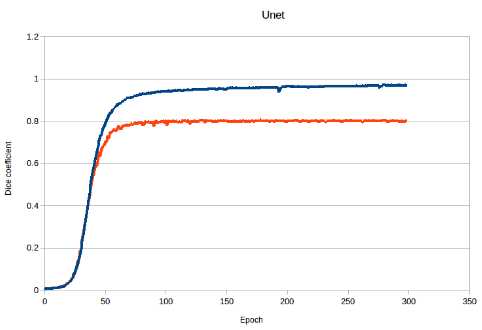
\includegraphics[width=\textwidth]{results/train_results_multi_unet.png}
% where an .eps filename suffix will be assumed under latex,
% and a .pdf suffix will be assumed for pdflatex
\caption{Multi label U-net training curve. Blue curve is training curve and the red curve is the validation curve. }
\label{fig:results_multi_unet_train}
\end{figure}

\begin{table}[tbh]
% increase table row spacing, adjust to taste
\renewcommand{\arraystretch}{1}
% if using array.sty, it might be a good idea to tweak the value of
% \extrarowheight as needed to properly center the text within the cells
\centering
% Some packages, such as MDW tools, offer better commands for making tables
% than the plain LaTeX2e tabular which is used here.
\begin{tabular}{|c|c|c|c|}
\hline
\textbf{Group} & \textbf{D03}& \textbf{D07}& \textbf{D28}\\
\hline
DFP & 0.816 & 0.724 & 0.771\\      
\hline
DZP & 0.813 & 0.825 & 0.792\\
\hline
MDZ & 0.818 & 0.782 & 0.777\\ 
\hline
VEH & 0.846 & 0.813 & 0.814\\ 
\hline
\end{tabular}
\caption{DSC scores of test data for multi label U-net}
\label{tab.multi_model_results_unet}
\end{table}

Figure ~\ref{fig:results_multi_unet_DFP}, ~\ref{fig:results_multi_unet_DZP}, ~\ref{fig:results_multi_unet_MDZ}, and ~\ref{fig:results_multi_unet_VEH} show the test results for multi label U-net for each of the different animals.
In slice 4 the cerebellum is modeled almost perfectly with every animal group which makes sense as it is the largest and one of the most distinct regions. 
The region is distinct because it has a clear boundary when it ends like the thalamus, but unlike the piriform cortex where the end of the region is determined by how much expertise someone has in the region. 
If there is no clear boundary it makes it not only harder for the model to distinguish where to segment, but it makes the training dataset subject to more variation by the person segmenting the ground truth. 
This is why for the prifiorm cortex regions on slice 31 we have a prediction for most the animals except for some of the VEH animal. 
One interesting region is the dorsolateral thalamus because of its shape change for different slices in the MRI image. slice 28 vs slice 31 have very different shapes for the dorsolateral thalamus. 



\begin{figure}[!htb]  
    \centering % <-- added
\begin{subfigure}{0.25\textwidth}
  \includegraphics[width=\linewidth]{results/multi-unet/"DFP01 R14-189-D03_4".png}
  \caption{D03 slice 4} 
\end{subfigure}\hfil % <-- added
\begin{subfigure}{0.25\textwidth}
  \includegraphics[width=\linewidth]{results/multi-unet/"DFP01 R14-189-D03_23".png}
  \caption{D03 slice 23}
\end{subfigure}\hfil % <-- added
\begin{subfigure}{0.25\textwidth}
  \includegraphics[width=\linewidth]{results/multi-unet/"DFP01 R14-189-D03_28".png}
  \caption{D03 slice 28}
\end{subfigure}\hfil % <-- added
\begin{subfigure}{0.25\textwidth}
  \includegraphics[width=\linewidth]{results/multi-unet/"DFP01 R14-189-D03_31".png}
  \caption{D03 slice 31}
\end{subfigure}


\medskip
\begin{subfigure}{0.25\textwidth}
  \includegraphics[width=\linewidth]{results/multi-unet/"DFP01 R14-189-D07_4".png}
  \caption{D07 slice 4}
\end{subfigure}\hfil % <-- added
\begin{subfigure}{0.25\textwidth}
  \includegraphics[width=\linewidth]{results/multi-unet/"DFP01 R14-189-D07_23".png}
  \caption{D07 slice 23}
\end{subfigure}\hfil % <-- added
\begin{subfigure}{0.25\textwidth}
  \includegraphics[width=\linewidth]{results/multi-unet/"DFP01 R14-189-D07_28".png}
  \caption{D07 slice 28}
\end{subfigure}\hfil % <-- added
\begin{subfigure}{0.25\textwidth}
  \includegraphics[width=\linewidth]{results/multi-unet/"DFP01 R14-189-D07_31".png}
  \caption{D07 slice 31}
\end{subfigure}


\medskip
\begin{subfigure}{0.25\textwidth}
  \includegraphics[width=\linewidth]{results/multi-unet/"DFP01 R14-189-D28_4".png}
  \caption{D28 slice 4}
\end{subfigure}\hfil % <-- added
\begin{subfigure}{0.25\textwidth}
  \includegraphics[width=\linewidth]{results/multi-unet/"DFP01 R14-189-D28_23".png}
  \caption{D28 slice 23}
\end{subfigure}\hfil % <-- added
\begin{subfigure}{0.25\textwidth}
  \includegraphics[width=\linewidth]{results/multi-unet/"DFP01 R14-189-D28_28".png}
  \caption{D28 slice 28}
\end{subfigure}\hfil % <-- added
\begin{subfigure}{0.25\textwidth}
  \includegraphics[width=\linewidth]{results/multi-unet/"DFP01 R14-189-D28_31".png}
  \caption{D28 slice 31}
\end{subfigure}
  
  \caption{Results for DFP animal group at day 3, day 7, day 28 on multi region U-net. The color regions are the predicted output the model sent and the blue region is the ground truth. Each color except blue represents a different region.}
  \label{fig:results_multi_unet_DFP}
\end{figure}




\begin{figure}[!htb]  
    \centering % <-- added
\begin{subfigure}{0.25\textwidth}
  \includegraphics[width=\linewidth]{results/multi-unet/"DZP01 R14-187-D03_4".png}
  \caption{D03 slice 4}
\end{subfigure}\hfil % <-- added
\begin{subfigure}{0.25\textwidth}
  \includegraphics[width=\linewidth]{results/multi-unet/"DZP01 R14-187-D03_23".png}
  \caption{D03 slice 23}
\end{subfigure}\hfil % <-- added
\begin{subfigure}{0.25\textwidth}
  \includegraphics[width=\linewidth]{results/multi-unet/"DZP01 R14-187-D03_28".png}
  \caption{D03 slice 28}
\end{subfigure}\hfil % <-- added
\begin{subfigure}{0.25\textwidth}
  \includegraphics[width=\linewidth]{results/multi-unet/"DZP01 R14-187-D03_31".png}
  \caption{D03 slice 31}
\end{subfigure}

\medskip
\begin{subfigure}{0.25\textwidth}
  \includegraphics[width=\linewidth]{results/multi-unet/"DZP01 R14-187-D07_4".png}
  \caption{D07 slice 4}
\end{subfigure}\hfil % <-- added
\begin{subfigure}{0.25\textwidth}
  \includegraphics[width=\linewidth]{results/multi-unet/"DZP01 R14-187-D07_23".png}
  \caption{D07 slice 23}
\end{subfigure}\hfil % <-- added
\begin{subfigure}{0.25\textwidth}
  \includegraphics[width=\linewidth]{results/multi-unet/"DZP01 R14-187-D07_28".png}
  \caption{D07 slice 28}
\end{subfigure}\hfil % <-- added
\begin{subfigure}{0.25\textwidth}
  \includegraphics[width=\linewidth]{results/multi-unet/"DZP01 R14-187-D07_31".png}
  \caption{D07 slice 31}
\end{subfigure}

\medskip
\begin{subfigure}{0.25\textwidth}
  \includegraphics[width=\linewidth]{results/multi-unet/"DZP01 R14-187-D28_4".png}
  \caption{D28 slice 4}
\end{subfigure}\hfil % <-- added
\begin{subfigure}{0.25\textwidth}
  \includegraphics[width=\linewidth]{results/multi-unet/"DZP01 R14-187-D28_23".png}
  \caption{D28 slice 23}
\end{subfigure}\hfil % <-- added
\begin{subfigure}{0.25\textwidth}
  \includegraphics[width=\linewidth]{results/multi-unet/"DZP01 R14-187-D28_28".png}
  \caption{D28 slice 28}
\end{subfigure}\hfil % <-- added
\begin{subfigure}{0.25\textwidth}
  \includegraphics[width=\linewidth]{results/multi-unet/"DZP01 R14-187-D28_31".png}
  \caption{D28 slice 31}
\end{subfigure}
  
  \caption{Results for DZP animal group at day 3, day 7, day 28 on multi region U-net. The color regions are the predicted output the model sent and the blue region is the ground truth. Each color except blue represents a different region.}
  \label{fig:results_multi_unet_DZP}
\end{figure}


\begin{figure}[!htb]  
    \centering % <-- added
\begin{subfigure}{0.25\textwidth}
  \includegraphics[width=\linewidth]{results/multi-unet/"MDZ01 R14-190-D03_4".png}
  \caption{D03 slice 4}
\end{subfigure}\hfil % <-- added
\begin{subfigure}{0.25\textwidth}
  \includegraphics[width=\linewidth]{results/multi-unet/"MDZ01 R14-190-D03_23".png}
  \caption{D03 slice 23}
\end{subfigure}\hfil % <-- added
\begin{subfigure}{0.25\textwidth}
  \includegraphics[width=\linewidth]{results/multi-unet/"MDZ01 R14-190-D03_28".png}
  \caption{D03 slice 28}
\end{subfigure}\hfil % <-- added
\begin{subfigure}{0.25\textwidth}
  \includegraphics[width=\linewidth]{results/multi-unet/"MDZ01 R14-190-D03_31".png}
  \caption{D03 slice 31}
\end{subfigure}

\medskip
\begin{subfigure}{0.25\textwidth}
  \includegraphics[width=\linewidth]{results/multi-unet/"MDZ01 R14-190-D07_4".png}
  \caption{D07 slice 4}
\end{subfigure}\hfil % <-- added
\begin{subfigure}{0.25\textwidth}
  \includegraphics[width=\linewidth]{results/multi-unet/"MDZ01 R14-190-D07_23".png}
  \caption{D07 slice 23}
\end{subfigure}\hfil % <-- added
\begin{subfigure}{0.25\textwidth}
  \includegraphics[width=\linewidth]{results/multi-unet/"MDZ01 R14-190-D07_28".png}
  \caption{D07 slice 28}
\end{subfigure}\hfil % <-- added
\begin{subfigure}{0.25\textwidth}
  \includegraphics[width=\linewidth]{results/multi-unet/"MDZ01 R14-190-D07_31".png}
  \caption{D07 slice 31}
\end{subfigure}

\medskip
\begin{subfigure}{0.25\textwidth}
  \includegraphics[width=\linewidth]{results/multi-unet/"MDZ01 R14-190-D28_4".png}
  \caption{D28 slice 4}
\end{subfigure}\hfil % <-- added
\begin{subfigure}{0.25\textwidth}
  \includegraphics[width=\linewidth]{results/multi-unet/"MDZ01 R14-190-D28_23".png}
  \caption{D28 slice 23}
\end{subfigure}\hfil % <-- added
\begin{subfigure}{0.25\textwidth}
  \includegraphics[width=\linewidth]{results/multi-unet/"MDZ01 R14-190-D28_28".png}
  \caption{D28 slice 28}
\end{subfigure}\hfil % <-- added
\begin{subfigure}{0.25\textwidth}
  \includegraphics[width=\linewidth]{results/multi-unet/"MDZ01 R14-190-D28_31".png}
  \caption{D28 slice 31}
\end{subfigure}
  
  \caption{Results for MDZ animal group at day 3, day 7, day 28 on multi region U-net. The color regions are the predicted output the model sent and the blue region is the ground truth. Each color except blue represents a different region.}
  \label{fig:results_multi_unet_MDZ}
\end{figure}



\begin{figure}[!htb]  
    \centering % <-- added
\begin{subfigure}{0.25\textwidth}
  \includegraphics[width=\linewidth]{results/multi-unet/"Veh01 R14-192-D03_4".png}
  \caption{D03 slice 4}
\end{subfigure}\hfil % <-- added
\begin{subfigure}{0.25\textwidth}
  \includegraphics[width=\linewidth]{results/multi-unet/"Veh01 R14-192-D03_23".png}
  \caption{D03 slice 23}
\end{subfigure}\hfil % <-- added
\begin{subfigure}{0.25\textwidth}
  \includegraphics[width=\linewidth]{results/multi-unet/"Veh01 R14-192-D03_28".png}
  \caption{D03 slice 28}
\end{subfigure}\hfil % <-- added
\begin{subfigure}{0.25\textwidth}
  \includegraphics[width=\linewidth]{results/multi-unet/"Veh01 R14-192-D03_31".png}
  \caption{D03 slice 31}
\end{subfigure}

\medskip
\begin{subfigure}{0.25\textwidth}
  \includegraphics[width=\linewidth]{results/multi-unet/"Veh01 R14-192-D07_4".png}
  \caption{D07 slice 4}
\end{subfigure}\hfil % <-- added
\begin{subfigure}{0.25\textwidth}
  \includegraphics[width=\linewidth]{results/multi-unet/"Veh01 R14-192-D07_23".png}
  \caption{D07 slice 23}
\end{subfigure}\hfil % <-- added
\begin{subfigure}{0.25\textwidth}
  \includegraphics[width=\linewidth]{results/multi-unet/"Veh01 R14-192-D07_28".png}
  \caption{D07 slice 28}
\end{subfigure}\hfil % <-- added
\begin{subfigure}{0.25\textwidth}
  \includegraphics[width=\linewidth]{results/multi-unet/"Veh01 R14-192-D07_31".png}
  \caption{D07 slice 31}
\end{subfigure}

\medskip
\begin{subfigure}{0.25\textwidth}
  \includegraphics[width=\linewidth]{results/multi-unet/"Veh01 R14-192-D28_4".png}
  \caption{D28 slice 4}
\end{subfigure}\hfil % <-- added
\begin{subfigure}{0.25\textwidth}
  \includegraphics[width=\linewidth]{results/multi-unet/"Veh01 R14-192-D28_23".png}
  \caption{D28 slice 23}
\end{subfigure}\hfil % <-- added
\begin{subfigure}{0.25\textwidth}
  \includegraphics[width=\linewidth]{results/multi-unet/"Veh01 R14-192-D28_28".png}
  \caption{D28 slice 28}
\end{subfigure}\hfil % <-- added
\begin{subfigure}{0.25\textwidth}
  \includegraphics[width=\linewidth]{results/multi-unet/"Veh01 R14-192-D28_31".png}
  \caption{D28 slice 31}
\end{subfigure}
  
  \caption{Results for VEH animal group at day 3, day 7, day 28 on multi region U-net. The color regions are the predicted output the model sent and the blue region is the ground truth. Each color except blue represents a different region.}
  \label{fig:results_multi_unet_VEH}
\end{figure}


\subsubsection{Modified Dilation VGG-16}
    Figure ~\ref{fig:results_multi_dilation_train} show the training results for the modified dilation VGG-16 model that was described before. 
    The training results were the worst for this model with the training and validation curves reaching a DSC of about 0.5.
    This could be due to the fact that the dilation VGG-16 model has the least amount of parameters as well as the fact that the batch size and filter size had to be reduced to 16 and the filter sizes had to be halved in order to be able to train. 
    Table ~\ref{tab.multi_model_results_dilation} shows the test data results for the model. The lowest DSC is the VEH group D07 where the dice score is 0.248. 
    The model didn't perform well on all the the different animal groups.
    We still see the correlation between the time points though with the earlier time points like D03 get higher DSC scores than the later time point images, but the difference is much smaller when compared to U-net. 
    This could mean that the dilation layers learn better from the later time points compared to U-net.
    
\begin{figure}[!tbh]
\centering
\includegraphics[width=\textwidth]{results/train_results_multi_dilation.png}
% where an .eps filename suffix will be assumed under latex,
% and a .pdf suffix will be assumed for pdflatex
\caption{Multi label dilation VGG-16 training curve. Blue curve is training curve and the red curve is the validation curve. }
\label{fig:results_multi_dilation_train}
\end{figure}

\begin{table}[tbh]
% increase table row spacing, adjust to taste
\renewcommand{\arraystretch}{1}
% if using array.sty, it might be a good idea to tweak the value of
% \extrarowheight as needed to properly center the text within the cells
\centering
% Some packages, such as MDW tools, offer better commands for making tables
% than the plain LaTeX2e tabular which is used here.
\begin{tabular}{|c|c|c|c|}
\hline
\textbf{Group} & \textbf{D03}& \textbf{D07}& \textbf{D28}\\
\hline
DFP & 0.488 & 0.472 & 0.429\\      
\hline
DZP & 0.495 & 0.533 & 0.466\\
\hline
MDZ & 0.487 & 0.504 & 0.468\\ 
\hline
VEH & 0.480 & 0.248 & 0.479\\ 
\hline
\end{tabular}
\caption{DSC scores of test data for multi label dilation VGG-16}
\label{tab.multi_model_results_dilation}
\end{table}


Figure ~\ref{fig:results_multi_dilation_DFP}, ~\ref{fig:results_multi_dilation_DZP}, ~\ref{fig:results_multi_dilation_MDZ}, and ~\ref{fig:results_multi_dilation_VEH} show the image results for the test data.
As shown in the images it seemed like only a certain amount of regions were predicted by the model. 
The cerebellum wasn't predicted by the model at all as well as many other regions. 
This means that the model only learned to segment some of the 14 different classes and wasn't trained well.
For the regions that were predicted like the right hippocampus and the inner and outer cerebral cortex they were predicted quite well. 
The reason that they DSC is so low is that since some of the regions aren't predicted it brings the average down.



\begin{figure}[!htb]  
    \centering % <-- added
\begin{subfigure}{0.25\textwidth}
  \includegraphics[width=\linewidth]{results/multi_dilation/"DFP01 R14-189-D03_4".png}
  \caption{D03 slice 4} 
\end{subfigure}\hfil % <-- added
\begin{subfigure}{0.25\textwidth}
  \includegraphics[width=\linewidth]{results/multi_dilation/"DFP01 R14-189-D03_23".png}
  \caption{D03 slice 23}
\end{subfigure}\hfil % <-- added
\begin{subfigure}{0.25\textwidth}
  \includegraphics[width=\linewidth]{results/multi_dilation/"DFP01 R14-189-D03_28".png}
  \caption{D03 slice 28}
\end{subfigure}\hfil % <-- added
\begin{subfigure}{0.25\textwidth}
  \includegraphics[width=\linewidth]{results/multi_dilation/"DFP01 R14-189-D03_31".png}
  \caption{D03 slice 31}
\end{subfigure}


\medskip
\begin{subfigure}{0.25\textwidth}
  \includegraphics[width=\linewidth]{results/multi_dilation/"DFP01 R14-189-D07_4".png}
  \caption{D07 slice 4}
\end{subfigure}\hfil % <-- added
\begin{subfigure}{0.25\textwidth}
  \includegraphics[width=\linewidth]{results/multi_dilation/"DFP01 R14-189-D07_23".png}
  \caption{D07 slice 23}
\end{subfigure}\hfil % <-- added
\begin{subfigure}{0.25\textwidth}
  \includegraphics[width=\linewidth]{results/multi_dilation/"DFP01 R14-189-D07_28".png}
  \caption{D07 slice 28}
\end{subfigure}\hfil % <-- added
\begin{subfigure}{0.25\textwidth}
  \includegraphics[width=\linewidth]{results/multi_dilation/"DFP01 R14-189-D07_31".png}
  \caption{D07 slice 31}
\end{subfigure}


\medskip
\begin{subfigure}{0.25\textwidth}
  \includegraphics[width=\linewidth]{results/multi_dilation/"DFP01 R14-189-D28_4".png}
  \caption{D28 slice 4}
\end{subfigure}\hfil % <-- added
\begin{subfigure}{0.25\textwidth}
  \includegraphics[width=\linewidth]{results/multi_dilation/"DFP01 R14-189-D28_23".png}
  \caption{D28 slice 23}
\end{subfigure}\hfil % <-- added
\begin{subfigure}{0.25\textwidth}
  \includegraphics[width=\linewidth]{results/multi_dilation/"DFP01 R14-189-D28_28".png}
  \caption{D28 slice 28}
\end{subfigure}\hfil % <-- added
\begin{subfigure}{0.25\textwidth}
  \includegraphics[width=\linewidth]{results/multi_dilation/"DFP01 R14-189-D28_31".png}
  \caption{D28 slice 31}
\end{subfigure}
  
  \caption{Results for DFP animal group at day 3, day 7, day 28 on multi region dilation VGG-16. The color regions are the predicted output the model sent and the blue region is the ground truth. Each color except blue represents a different region.}
  \label{fig:results_multi_dilation_DFP}
\end{figure}




\begin{figure}[!htb]  
    \centering % <-- added
\begin{subfigure}{0.25\textwidth}
  \includegraphics[width=\linewidth]{results/multi_dilation/"DZP01 R14-187-D03_4".png}
  \caption{D03 slice 4}
\end{subfigure}\hfil % <-- added
\begin{subfigure}{0.25\textwidth}
  \includegraphics[width=\linewidth]{results/multi_dilation/"DZP01 R14-187-D03_23".png}
  \caption{D03 slice 23}
\end{subfigure}\hfil % <-- added
\begin{subfigure}{0.25\textwidth}
  \includegraphics[width=\linewidth]{results/multi_dilation/"DZP01 R14-187-D03_28".png}
  \caption{D03 slice 28}
\end{subfigure}\hfil % <-- added
\begin{subfigure}{0.25\textwidth}
  \includegraphics[width=\linewidth]{results/multi_dilation/"DZP01 R14-187-D03_31".png}
  \caption{D03 slice 31}
\end{subfigure}

\medskip
\begin{subfigure}{0.25\textwidth}
  \includegraphics[width=\linewidth]{results/multi_dilation/"DZP01 R14-187-D07_4".png}
  \caption{D07 slice 4}
\end{subfigure}\hfil % <-- added
\begin{subfigure}{0.25\textwidth}
  \includegraphics[width=\linewidth]{results/multi_dilation/"DZP01 R14-187-D07_23".png}
  \caption{D07 slice 23}
\end{subfigure}\hfil % <-- added
\begin{subfigure}{0.25\textwidth}
  \includegraphics[width=\linewidth]{results/multi_dilation/"DZP01 R14-187-D07_28".png}
  \caption{D07 slice 28}
\end{subfigure}\hfil % <-- added
\begin{subfigure}{0.25\textwidth}
  \includegraphics[width=\linewidth]{results/multi_dilation/"DZP01 R14-187-D07_31".png}
  \caption{D07 slice 31}
\end{subfigure}

\medskip
\begin{subfigure}{0.25\textwidth}
  \includegraphics[width=\linewidth]{results/multi_dilation/"DZP01 R14-187-D28_4".png}
  \caption{D28 slice 4}
\end{subfigure}\hfil % <-- added
\begin{subfigure}{0.25\textwidth}
  \includegraphics[width=\linewidth]{results/multi_dilation/"DZP01 R14-187-D28_23".png}
  \caption{D28 slice 23}
\end{subfigure}\hfil % <-- added
\begin{subfigure}{0.25\textwidth}
  \includegraphics[width=\linewidth]{results/multi_dilation/"DZP01 R14-187-D28_28".png}
  \caption{D28 slice 28}
\end{subfigure}\hfil % <-- added
\begin{subfigure}{0.25\textwidth}
  \includegraphics[width=\linewidth]{results/multi_dilation/"DZP01 R14-187-D28_31".png}
  \caption{D28 slice 31}
\end{subfigure}
  
  \caption{Results for DZP animal group at day 3, day 7, day 28 on multi region dilation VGG-16. The color regions are the predicted output the model sent and the blue region is the ground truth. Each color except blue represents a different region.}
  \label{fig:results_multi_dilation_DZP}
\end{figure}


\begin{figure}[!htb]  
    \centering % <-- added
\begin{subfigure}{0.25\textwidth}
  \includegraphics[width=\linewidth]{results/multi_dilation/"MDZ01 R14-190-D03_4".png}
  \caption{D03 slice 4}
\end{subfigure}\hfil % <-- added
\begin{subfigure}{0.25\textwidth}
  \includegraphics[width=\linewidth]{results/multi_dilation/"MDZ01 R14-190-D03_23".png}
  \caption{D03 slice 23}
\end{subfigure}\hfil % <-- added
\begin{subfigure}{0.25\textwidth}
  \includegraphics[width=\linewidth]{results/multi_dilation/"MDZ01 R14-190-D03_28".png}
  \caption{D03 slice 28}
\end{subfigure}\hfil % <-- added
\begin{subfigure}{0.25\textwidth}
  \includegraphics[width=\linewidth]{results/multi_dilation/"MDZ01 R14-190-D03_31".png}
  \caption{D03 slice 31}
\end{subfigure}

\medskip
\begin{subfigure}{0.25\textwidth}
  \includegraphics[width=\linewidth]{results/multi_dilation/"MDZ01 R14-190-D07_4".png}
  \caption{D07 slice 4}
\end{subfigure}\hfil % <-- added
\begin{subfigure}{0.25\textwidth}
  \includegraphics[width=\linewidth]{results/multi_dilation/"MDZ01 R14-190-D07_23".png}
  \caption{D07 slice 23}
\end{subfigure}\hfil % <-- added
\begin{subfigure}{0.25\textwidth}
  \includegraphics[width=\linewidth]{results/multi_dilation/"MDZ01 R14-190-D07_28".png}
  \caption{D07 slice 28}
\end{subfigure}\hfil % <-- added
\begin{subfigure}{0.25\textwidth}
  \includegraphics[width=\linewidth]{results/multi_dilation/"MDZ01 R14-190-D07_31".png}
  \caption{D07 slice 31}
\end{subfigure}

\medskip
\begin{subfigure}{0.25\textwidth}
  \includegraphics[width=\linewidth]{results/multi_dilation/"MDZ01 R14-190-D28_4".png}
  \caption{D28 slice 4}
\end{subfigure}\hfil % <-- added
\begin{subfigure}{0.25\textwidth}
  \includegraphics[width=\linewidth]{results/multi_dilation/"MDZ01 R14-190-D28_23".png}
  \caption{D28 slice 23}
\end{subfigure}\hfil % <-- added
\begin{subfigure}{0.25\textwidth}
  \includegraphics[width=\linewidth]{results/multi_dilation/"MDZ01 R14-190-D28_28".png}
  \caption{D28 slice 28}
\end{subfigure}\hfil % <-- added
\begin{subfigure}{0.25\textwidth}
  \includegraphics[width=\linewidth]{results/multi_dilation/"MDZ01 R14-190-D28_31".png}
  \caption{D28 slice 31}
\end{subfigure}
  
  \caption{Results for MDZ animal group at day 3, day 7, day 28 on multi region dilation VGG-16. The color regions are the predicted output the model sent and the blue region is the ground truth. Each color except blue represents a different region.}
  \label{fig:results_multi_dilation_MDZ}
\end{figure}



\begin{figure}[!htb]  
    \centering % <-- added
\begin{subfigure}{0.25\textwidth}
  \includegraphics[width=\linewidth]{results/multi_dilation/"Veh01 R14-192-D03_4".png}
  \caption{D03 slice 4}
\end{subfigure}\hfil % <-- added
\begin{subfigure}{0.25\textwidth}
  \includegraphics[width=\linewidth]{results/multi_dilation/"Veh01 R14-192-D03_23".png}
  \caption{D03 slice 23}
\end{subfigure}\hfil % <-- added
\begin{subfigure}{0.25\textwidth}
  \includegraphics[width=\linewidth]{results/multi_dilation/"Veh01 R14-192-D03_28".png}
  \caption{D03 slice 28}
\end{subfigure}\hfil % <-- added
\begin{subfigure}{0.25\textwidth}
  \includegraphics[width=\linewidth]{results/multi_dilation/"Veh01 R14-192-D03_31".png}
  \caption{D03 slice 31}
\end{subfigure}

\medskip
\begin{subfigure}{0.25\textwidth}
  \includegraphics[width=\linewidth]{results/multi_dilation/"Veh01 R14-192-D07_4".png}
  \caption{D07 slice 4}
\end{subfigure}\hfil % <-- added
\begin{subfigure}{0.25\textwidth}
  \includegraphics[width=\linewidth]{results/multi_dilation/"Veh01 R14-192-D07_23".png}
  \caption{D07 slice 23}
\end{subfigure}\hfil % <-- added
\begin{subfigure}{0.25\textwidth}
  \includegraphics[width=\linewidth]{results/multi_dilation/"Veh01 R14-192-D07_28".png}
  \caption{D07 slice 28}
\end{subfigure}\hfil % <-- added
\begin{subfigure}{0.25\textwidth}
  \includegraphics[width=\linewidth]{results/multi_dilation/"Veh01 R14-192-D07_31".png}
  \caption{D07 slice 31}
\end{subfigure}

\medskip
\begin{subfigure}{0.25\textwidth}
  \includegraphics[width=\linewidth]{results/multi_dilation/"Veh01 R14-192-D28_4".png}
  \caption{D28 slice 4}
\end{subfigure}\hfil % <-- added
\begin{subfigure}{0.25\textwidth}
  \includegraphics[width=\linewidth]{results/multi_dilation/"Veh01 R14-192-D28_23".png}
  \caption{D28 slice 23}
\end{subfigure}\hfil % <-- added
\begin{subfigure}{0.25\textwidth}
  \includegraphics[width=\linewidth]{results/multi_dilation/"Veh01 R14-192-D28_28".png}
  \caption{D28 slice 28}
\end{subfigure}\hfil % <-- added
\begin{subfigure}{0.25\textwidth}
  \includegraphics[width=\linewidth]{results/multi_dilation/"Veh01 R14-192-D28_31".png}
  \caption{D28 slice 31}
\end{subfigure}
  
  \caption{Results for VEH animal group at day 3, day 7, day 28 on multi region dilation VGG-16. The color regions are the predicted output the model sent and the blue region is the ground truth. Each color except blue represents a different region.}
  \label{fig:results_multi_dilation_VEH}
\end{figure}


\subsubsection{U-net Dilation 2 downsampling}
    These are the results for the combination of U-net and the dilation contextual layers using two downsampling layers. Figure ~\ref{fig:results_multi_unetdil2_train} shows the training results for the model.
    This curve at first shows the training curve to be lower than the validation curve, but later on the training curve increases significantly while the validation curve mainly stays the same. 
    This can be explained because of the data augmentation that was used. Since the training dataset was much more complex than the validation dataset then the model took longer to learn the training images. 
    Table ~\ref{tab.multi_model_results_unetdil2} shows the results of the model on the test dataset for each animal group and day. 
    Overall this model performs very well which the highest DSC attributed to the VEH animal group and the lowest DSC scores associated with the DFP animal group. 
    This means that the model was able to learn well with the more consistent VEH group, but when it tried to learn the vastly different DFP group it wasn't able to perform as well. 
    We also see a correlation where the later the MRI images were taken the lower the DSC, except with the DZP animal group. 
    When we compare this to the U-net DSC scores we see that even though this model performs very well U-net performs slightly better overall for almost all of the time points. 

\begin{figure}[!tbh]
\centering
\includegraphics[width=\textwidth]{results/train_results_multi_unetdil2.png}
% where an .eps filename suffix will be assumed under latex,
% and a .pdf suffix will be assumed for pdflatex
\caption{Multi label U-net dilation 2 downsampling training curve. Blue curve is training curve and the red curve is the validation curve. }
\label{fig:results_multi_unetdil2_train}
\end{figure}

\begin{table}[tbh]
% increase table row spacing, adjust to taste
\renewcommand{\arraystretch}{1}
% if using array.sty, it might be a good idea to tweak the value of
% \extrarowheight as needed to properly center the text within the cells
\centering
% Some packages, such as MDW tools, offer better commands for making tables
% than the plain LaTeX2e tabular which is used here.
\begin{tabular}{|c|c|c|c|}
\hline
\textbf{Group} & \textbf{D03}& \textbf{D07}& \textbf{D28}\\
\hline
DFP & 0.780 & 0.759 & 0.743\\      
\hline
DZP & 0.765 & 0.835 & 0.798\\
\hline
MDZ & 0.800 & 0.772 & 0.750\\ 
\hline
VEH & 0.833 & 0.830 & 0.813\\ 
\hline
\end{tabular}
\caption{DSC scores of test data for multi label U-net dilation 2 downsampling}
\label{tab.multi_model_results_unetdil2}
\end{table}

Figure ~\ref{fig:results_multi_unetdil2_DFP}, ~\ref{fig:results_multi_unetdil2_DZP}, ~\ref{fig:results_multi_unetdil2_MDZ}, and ~\ref{fig:results_multi_unetdil2_VEH} show the image results for the U-net dilation combination model. 
We see once again that for the smaller regions the segmentation becomes worse with the medial thalamus in slice 28 D07 not being predicted or the dorsolateral thalamus being predicted but smaller than usual or off to the side from the ground truth for D07 or D28. 
In each of the days the regions change significantly where in D03 silce 28 the medial thalamus isn't there, but returns in the later time points.
This inconsistency hinders the model from performing better and counteracts the images that it has learned beforhand. 
This inconsistency though only happens with the either beginning or end of the region in z space and the middle regions for the animals are consistently segmented well. 
The change in the images between the segmentation of the animal groups can also be shown in figure ~\ref{fig:results_multi_unetdil2_DFP} and ~\ref{fig:results_multi_unetdil2_VEH}.
Since the images change significantly in figure ~\ref{fig:results_multi_unetdil2_DFP} the segmentation isn't as consistent with the dorsolateral thalamus as well especially as the images change from D03 to D28.
On comparison figure ~\ref{fig:results_multi_unetdil2_VEH} shows that as the MRI's change from D03 to D28 then the results are manly consistent between them with only the minor segmentation differences between them. 


\begin{figure}[!htb]  
    \centering % <-- added
\begin{subfigure}{0.25\textwidth}
  \includegraphics[width=\linewidth]{results/multi_unet_dil_2/"DFP01 R14-189-D03_4".png}
  \caption{D03 slice 4} 
\end{subfigure}\hfil % <-- added
\begin{subfigure}{0.25\textwidth}
  \includegraphics[width=\linewidth]{results/multi_unet_dil_2/"DFP01 R14-189-D03_23".png}
  \caption{D03 slice 23}
\end{subfigure}\hfil % <-- added
\begin{subfigure}{0.25\textwidth}
  \includegraphics[width=\linewidth]{results/multi_unet_dil_2/"DFP01 R14-189-D03_28".png}
  \caption{D03 slice 28}
\end{subfigure}\hfil % <-- added
\begin{subfigure}{0.25\textwidth}
  \includegraphics[width=\linewidth]{results/multi_unet_dil_2/"DFP01 R14-189-D03_31".png}
  \caption{D03 slice 31}
\end{subfigure}


\medskip
\begin{subfigure}{0.25\textwidth}
  \includegraphics[width=\linewidth]{results/multi_unet_dil_2/"DFP01 R14-189-D07_4".png}
  \caption{D07 slice 4}
\end{subfigure}\hfil % <-- added
\begin{subfigure}{0.25\textwidth}
  \includegraphics[width=\linewidth]{results/multi_unet_dil_2/"DFP01 R14-189-D07_23".png}
  \caption{D07 slice 23}
\end{subfigure}\hfil % <-- added
\begin{subfigure}{0.25\textwidth}
  \includegraphics[width=\linewidth]{results/multi_unet_dil_2/"DFP01 R14-189-D07_28".png}
  \caption{D07 slice 28}
\end{subfigure}\hfil % <-- added
\begin{subfigure}{0.25\textwidth}
  \includegraphics[width=\linewidth]{results/multi_unet_dil_2/"DFP01 R14-189-D07_31".png}
  \caption{D07 slice 31}
\end{subfigure}


\medskip
\begin{subfigure}{0.25\textwidth}
  \includegraphics[width=\linewidth]{results/multi_unet_dil_2/"DFP01 R14-189-D28_4".png}
  \caption{D28 slice 4}
\end{subfigure}\hfil % <-- added
\begin{subfigure}{0.25\textwidth}
  \includegraphics[width=\linewidth]{results/multi_unet_dil_2/"DFP01 R14-189-D28_23".png}
  \caption{D28 slice 23}
\end{subfigure}\hfil % <-- added
\begin{subfigure}{0.25\textwidth}
  \includegraphics[width=\linewidth]{results/multi_unet_dil_2/"DFP01 R14-189-D28_28".png}
  \caption{D28 slice 28}
\end{subfigure}\hfil % <-- added
\begin{subfigure}{0.25\textwidth}
  \includegraphics[width=\linewidth]{results/multi_unet_dil_2/"DFP01 R14-189-D28_31".png}
  \caption{D28 slice 31}
\end{subfigure}
  
  \caption{Results for DFP animal group at day 3, day 7, day 28 on multi region U-net dilation 2 downsampling. The color regions are the predicted output the model sent and the blue region is the ground truth. Each color except blue represents a different region.}
  \label{fig:results_multi_unetdil2_DFP}
\end{figure}




\begin{figure}[!htb]  
    \centering % <-- added
\begin{subfigure}{0.25\textwidth}
  \includegraphics[width=\linewidth]{results/multi_unet_dil_2/"DZP01 R14-187-D03_4".png}
  \caption{D03 slice 4}
\end{subfigure}\hfil % <-- added
\begin{subfigure}{0.25\textwidth}
  \includegraphics[width=\linewidth]{results/multi_unet_dil_2/"DZP01 R14-187-D03_23".png}
  \caption{D03 slice 23}
\end{subfigure}\hfil % <-- added
\begin{subfigure}{0.25\textwidth}
  \includegraphics[width=\linewidth]{results/multi_unet_dil_2/"DZP01 R14-187-D03_28".png}
  \caption{D03 slice 28}
\end{subfigure}\hfil % <-- added
\begin{subfigure}{0.25\textwidth}
  \includegraphics[width=\linewidth]{results/multi_unet_dil_2/"DZP01 R14-187-D03_31".png}
  \caption{D03 slice 31}
\end{subfigure}

\medskip
\begin{subfigure}{0.25\textwidth}
  \includegraphics[width=\linewidth]{results/multi_unet_dil_2/"DZP01 R14-187-D07_4".png}
  \caption{D07 slice 4}
\end{subfigure}\hfil % <-- added
\begin{subfigure}{0.25\textwidth}
  \includegraphics[width=\linewidth]{results/multi_unet_dil_2/"DZP01 R14-187-D07_23".png}
  \caption{D07 slice 23}
\end{subfigure}\hfil % <-- added
\begin{subfigure}{0.25\textwidth}
  \includegraphics[width=\linewidth]{results/multi_unet_dil_2/"DZP01 R14-187-D07_28".png}
  \caption{D07 slice 28}
\end{subfigure}\hfil % <-- added
\begin{subfigure}{0.25\textwidth}
  \includegraphics[width=\linewidth]{results/multi_unet_dil_2/"DZP01 R14-187-D07_31".png}
  \caption{D07 slice 31}
\end{subfigure}

\medskip
\begin{subfigure}{0.25\textwidth}
  \includegraphics[width=\linewidth]{results/multi_unet_dil_2/"DZP01 R14-187-D28_4".png}
  \caption{D28 slice 4}
\end{subfigure}\hfil % <-- added
\begin{subfigure}{0.25\textwidth}
  \includegraphics[width=\linewidth]{results/multi_unet_dil_2/"DZP01 R14-187-D28_23".png}
  \caption{D28 slice 23}
\end{subfigure}\hfil % <-- added
\begin{subfigure}{0.25\textwidth}
  \includegraphics[width=\linewidth]{results/multi_unet_dil_2/"DZP01 R14-187-D28_28".png}
  \caption{D28 slice 28}
\end{subfigure}\hfil % <-- added
\begin{subfigure}{0.25\textwidth}
  \includegraphics[width=\linewidth]{results/multi_unet_dil_2/"DZP01 R14-187-D28_31".png}
  \caption{D28 slice 31}
\end{subfigure}
  
  \caption{Results for DZP animal group at day 3, day 7, day 28 on multi region U-net dilation 2 downsampling. The color regions are the predicted output the model sent and the blue region is the ground truth. Each color except blue represents a different region.}
  \label{fig:results_multi_unetdil2_DZP}
\end{figure}


\begin{figure}[!htb]  
    \centering % <-- added
\begin{subfigure}{0.25\textwidth}
  \includegraphics[width=\linewidth]{results/multi_unet_dil_2/"MDZ01 R14-190-D03_4".png}
  \caption{D03 slice 4}
\end{subfigure}\hfil % <-- added
\begin{subfigure}{0.25\textwidth}
  \includegraphics[width=\linewidth]{results/multi_unet_dil_2/"MDZ01 R14-190-D03_23".png}
  \caption{D03 slice 23}
\end{subfigure}\hfil % <-- added
\begin{subfigure}{0.25\textwidth}
  \includegraphics[width=\linewidth]{results/multi_unet_dil_2/"MDZ01 R14-190-D03_28".png}
  \caption{D03 slice 28}
\end{subfigure}\hfil % <-- added
\begin{subfigure}{0.25\textwidth}
  \includegraphics[width=\linewidth]{results/multi_unet_dil_2/"MDZ01 R14-190-D03_31".png}
  \caption{D03 slice 31}
\end{subfigure}

\medskip
\begin{subfigure}{0.25\textwidth}
  \includegraphics[width=\linewidth]{results/multi_unet_dil_2/"MDZ01 R14-190-D07_4".png}
  \caption{D07 slice 4}
\end{subfigure}\hfil % <-- added
\begin{subfigure}{0.25\textwidth}
  \includegraphics[width=\linewidth]{results/multi_unet_dil_2/"MDZ01 R14-190-D07_23".png}
  \caption{D07 slice 23}
\end{subfigure}\hfil % <-- added
\begin{subfigure}{0.25\textwidth}
  \includegraphics[width=\linewidth]{results/multi_unet_dil_2/"MDZ01 R14-190-D07_28".png}
  \caption{D07 slice 28}
\end{subfigure}\hfil % <-- added
\begin{subfigure}{0.25\textwidth}
  \includegraphics[width=\linewidth]{results/multi_unet_dil_2/"MDZ01 R14-190-D07_31".png}
  \caption{D07 slice 31}
\end{subfigure}

\medskip
\begin{subfigure}{0.25\textwidth}
  \includegraphics[width=\linewidth]{results/multi_unet_dil_2/"MDZ01 R14-190-D28_4".png}
  \caption{D28 slice 4}
\end{subfigure}\hfil % <-- added
\begin{subfigure}{0.25\textwidth}
  \includegraphics[width=\linewidth]{results/multi_unet_dil_2/"MDZ01 R14-190-D28_23".png}
  \caption{D28 slice 23}
\end{subfigure}\hfil % <-- added
\begin{subfigure}{0.25\textwidth}
  \includegraphics[width=\linewidth]{results/multi_unet_dil_2/"MDZ01 R14-190-D28_28".png}
  \caption{D28 slice 28}
\end{subfigure}\hfil % <-- added
\begin{subfigure}{0.25\textwidth}
  \includegraphics[width=\linewidth]{results/multi_unet_dil_2/"MDZ01 R14-190-D28_31".png}
  \caption{D28 slice 31}
\end{subfigure}
  
  \caption{Results for MDZ animal group at day 3, day 7, day 28 on multi region U-net dilation 2 downsampling. The color regions are the predicted output the model sent and the blue region is the ground truth. Each color except blue represents a different region.}
  \label{fig:results_multi_unetdil2_MDZ}
\end{figure}



\begin{figure}[!htb]  
    \centering % <-- added
\begin{subfigure}{0.25\textwidth}
  \includegraphics[width=\linewidth]{results/multi_unet_dil_2/"Veh02 R14-200-D03_4".png}
  \caption{D03 slice 4}
\end{subfigure}\hfil % <-- added
\begin{subfigure}{0.25\textwidth}
  \includegraphics[width=\linewidth]{results/multi_unet_dil_2/"Veh02 R14-200-D03_23".png}
  \caption{D03 slice 23}
\end{subfigure}\hfil % <-- added
\begin{subfigure}{0.25\textwidth}
  \includegraphics[width=\linewidth]{results/multi_unet_dil_2/"Veh02 R14-200-D03_28".png}
  \caption{D03 slice 28}
\end{subfigure}\hfil % <-- added
\begin{subfigure}{0.25\textwidth}
  \includegraphics[width=\linewidth]{results/multi_unet_dil_2/"Veh02 R14-200-D03_31".png}
  \caption{D03 slice 31}
\end{subfigure}

\medskip
\begin{subfigure}{0.25\textwidth}
  \includegraphics[width=\linewidth]{results/multi_unet_dil_2/"Veh02 R14-200-D07_4".png}
  \caption{D07 slice 4}
\end{subfigure}\hfil % <-- added
\begin{subfigure}{0.25\textwidth}
  \includegraphics[width=\linewidth]{results/multi_unet_dil_2/"Veh02 R14-200-D07_23".png}
  \caption{D07 slice 23}
\end{subfigure}\hfil % <-- added
\begin{subfigure}{0.25\textwidth}
  \includegraphics[width=\linewidth]{results/multi_unet_dil_2/"Veh02 R14-200-D07_28".png}
  \caption{D07 slice 28}
\end{subfigure}\hfil % <-- added
\begin{subfigure}{0.25\textwidth}
  \includegraphics[width=\linewidth]{results/multi_unet_dil_2/"Veh02 R14-200-D07_31".png}
  \caption{D07 slice 31}
\end{subfigure}

\medskip
\begin{subfigure}{0.25\textwidth}
  \includegraphics[width=\linewidth]{results/multi_unet_dil_2/"Veh02 R14-200-D28_4".png}
  \caption{D28 slice 4}
\end{subfigure}\hfil % <-- added
\begin{subfigure}{0.25\textwidth}
  \includegraphics[width=\linewidth]{results/multi_unet_dil_2/"Veh02 R14-200-D28_23".png}
  \caption{D28 slice 23}
\end{subfigure}\hfil % <-- added
\begin{subfigure}{0.25\textwidth}
  \includegraphics[width=\linewidth]{results/multi_unet_dil_2/"Veh02 R14-200-D28_28".png}
  \caption{D28 slice 28}
\end{subfigure}\hfil % <-- added
\begin{subfigure}{0.25\textwidth}
  \includegraphics[width=\linewidth]{results/multi_unet_dil_2/"Veh02 R14-200-D28_31".png}
  \caption{D28 slice 31}
\end{subfigure}
  
  \caption{Results for VEH animal group at day 3, day 7, day 28 on multi region U-net dilation 2 downsampling. The color regions are the predicted output the model sent and the blue region is the ground truth. Each color except blue represents a different region.}
  \label{fig:results_multi_unetdil2_VEH}
\end{figure}



\subsubsection{U-net Dilation 3 downsampling}
These are the results for the U-net dilation contextual layers combination but with 3 dowsnsamlping layers instead. 
Figure ~\ref{fig:results_multi_unetdil3_train} shows the training results for this model.
One interesting thing that was said for U-net dilation 2 downsampling was that the training curve started out lower and slowly increased until it ended at around 0.85 for training and at around 0.79 for validation. 
For the U-net dilation 3 downsampling model the training curve increases much slower, but starts at around the same area.
This can also be attributed to the increased complexity of the training dataset and the minor increase in the number of parameters from the increased layer. 
The curve increasing slower than the 2 downsampling model is due the idea that since the model is deeper it has a million more parameters that need to be trained and changed and so after a certain point the training is slowed.
This could also be due the inconsistencies pulling the model in opposite directions and training slower. 
Even though the model was harder to train though the model performed better on the validation data ending up at around 0.82. 
Table ~\ref{tab.multi_model_results_unetdil3} shows the results for the test image dataset. 
The patterns seen in the unet dilation 2 downsampling is also seen here, where VEH animal group performs the best and that the usually as the day increases the DSC scores decrease. 
This model though overall performs better than U-net especially for the later time point data like D28 and D07.
U-net is originally 3 downsampling layers and so the inclusion of the dilation contextual layer block at the bottom of the downsampling layers helped the model to learn more from the later time points. 


\begin{figure}[!tbh]
\centering
\includegraphics[width=\textwidth]{results/train_results_multi_unetdil3.png}
% where an .eps filename suffix will be assumed under latex,
% and a .pdf suffix will be assumed for pdflatex
\caption{Multi label U-net dilation 3 downsampling training curve. Blue curve is training curve and the red curve is the validation curve. }
\label{fig:results_multi_unetdil3_train}
\end{figure}

\begin{table}[tbh]
% increase table row spacing, adjust to taste
\renewcommand{\arraystretch}{1}
% if using array.sty, it might be a good idea to tweak the value of
% \extrarowheight as needed to properly center the text within the cells
\centering
% Some packages, such as MDW tools, offer better commands for making tables
% than the plain LaTeX2e tabular which is used here.
\begin{tabular}{|c|c|c|c|}
\hline
\textbf{Group} & \textbf{D03}& \textbf{D07}& \textbf{D28}\\
\hline
DFP & 0.813 & 0.765 & 0.784\\      
\hline
DZP & 0.774 & 0.854 & 0.819\\
\hline
MDZ & 0.818 & 0.797 & 0.786\\ 
\hline
VEH & 0.851 & 0.841 & 0.842\\ 
\hline
\end{tabular}
\caption{DSC scores of test data for multi label U-net dilation 3 downsampling}
\label{tab.multi_model_results_unetdil3}
\end{table}


Figure ~\ref{fig:results_multi_unetdil3_DFP}, ~\ref{fig:results_multi_unetdil3_DZP}, ~\ref{fig:results_multi_unetdil3_MDZ}, and ~\ref{fig:results_multi_unetdil3_VEH} show segmentation for the test image dataset. 
Overall the model is able to segment the regions quite well, the smaller regions though still have the most trouble by the model. 
The model also still has problems with the prifiorm cortex which is one of the hardest as it has no defined space within the MRI image.
The model though models the inner and outer cerebral cortex quite well like in D28 slice 31 it is able to predict the regions quite well when other models had trouble with this.
Figure ~\ref{fig:results_multi_unetdil3_DFP} at slice 28 the model has the most trouble with medial and dorsolateral thalamus.
The model also puts a preference on predicting the VEH animals as seen in figure ~\ref{fig:results_multi_unetdil3_VEH}.
An example is the inner and outer cerebral cortex D03 and D28 where the model correctly predicts no cortex on D03 slice 23 and correctly predicts the cerebral cortex in D28 slice 31. In the other animal groups like MDZ or the DZP the model makes the mistake of not predicting the cerebral cortex in D03 slice 23. 
This is the same with the piriform cortex as well where in the VEH animal group the piriform cortex was correctly predicted in slice 31, but for the other animal groups that didn't have the piriform cortex in slice 31, the model still predicted something.

\begin{figure}[!htb]  
    \centering % <-- added
\begin{subfigure}{0.25\textwidth}
  \includegraphics[width=\linewidth]{results/multi_unet_dil_3/"DFP01 R14-189-D03_4".png}
  \caption{D03 slice 4} 
\end{subfigure}\hfil % <-- added
\begin{subfigure}{0.25\textwidth}
  \includegraphics[width=\linewidth]{results/multi_unet_dil_3/"DFP01 R14-189-D03_23".png}
  \caption{D03 slice 23}
\end{subfigure}\hfil % <-- added
\begin{subfigure}{0.25\textwidth}
  \includegraphics[width=\linewidth]{results/multi_unet_dil_3/"DFP01 R14-189-D03_28".png}
  \caption{D03 slice 28}
\end{subfigure}\hfil % <-- added
\begin{subfigure}{0.25\textwidth}
  \includegraphics[width=\linewidth]{results/multi_unet_dil_3/"DFP01 R14-189-D03_31".png}
  \caption{D03 slice 31}
\end{subfigure}


\medskip
\begin{subfigure}{0.25\textwidth}
  \includegraphics[width=\linewidth]{results/multi_unet_dil_3/"DFP01 R14-189-D07_4".png}
  \caption{D07 slice 4}
\end{subfigure}\hfil % <-- added
\begin{subfigure}{0.25\textwidth}
  \includegraphics[width=\linewidth]{results/multi_unet_dil_3/"DFP01 R14-189-D07_23".png}
  \caption{D07 slice 23}
\end{subfigure}\hfil % <-- added
\begin{subfigure}{0.25\textwidth}
  \includegraphics[width=\linewidth]{results/multi_unet_dil_3/"DFP01 R14-189-D07_28".png}
  \caption{D07 slice 28}
\end{subfigure}\hfil % <-- added
\begin{subfigure}{0.25\textwidth}
  \includegraphics[width=\linewidth]{results/multi_unet_dil_3/"DFP01 R14-189-D07_31".png}
  \caption{D07 slice 31}
\end{subfigure}


\medskip
\begin{subfigure}{0.25\textwidth}
  \includegraphics[width=\linewidth]{results/multi_unet_dil_3/"DFP01 R14-189-D28_4".png}
  \caption{D28 slice 4}
\end{subfigure}\hfil % <-- added
\begin{subfigure}{0.25\textwidth}
  \includegraphics[width=\linewidth]{results/multi_unet_dil_3/"DFP01 R14-189-D28_23".png}
  \caption{D28 slice 23}
\end{subfigure}\hfil % <-- added
\begin{subfigure}{0.25\textwidth}
  \includegraphics[width=\linewidth]{results/multi_unet_dil_3/"DFP01 R14-189-D28_28".png}
  \caption{D28 slice 28}
\end{subfigure}\hfil % <-- added
\begin{subfigure}{0.25\textwidth}
  \includegraphics[width=\linewidth]{results/multi_unet_dil_3/"DFP01 R14-189-D28_31".png}
  \caption{D28 slice 31}
\end{subfigure}
  
  \caption{Results for DFP animal group at day 3, day 7, day 28 on multi region U-net dilation 3 downsampling. The color regions are the predicted output the model sent and the blue region is the ground truth. Each color except blue represents a different region.}
  \label{fig:results_multi_unetdil3_DFP}
\end{figure}




\begin{figure}[!htb]  
    \centering % <-- added
\begin{subfigure}{0.25\textwidth}
  \includegraphics[width=\linewidth]{results/multi_unet_dil_3/"DZP01 R14-187-D03_4".png}
  \caption{D03 slice 4}
\end{subfigure}\hfil % <-- added
\begin{subfigure}{0.25\textwidth}
  \includegraphics[width=\linewidth]{results/multi_unet_dil_3/"DZP01 R14-187-D03_23".png}
  \caption{D03 slice 23}
\end{subfigure}\hfil % <-- added
\begin{subfigure}{0.25\textwidth}
  \includegraphics[width=\linewidth]{results/multi_unet_dil_3/"DZP01 R14-187-D03_28".png}
  \caption{D03 slice 28}
\end{subfigure}\hfil % <-- added
\begin{subfigure}{0.25\textwidth}
  \includegraphics[width=\linewidth]{results/multi_unet_dil_3/"DZP01 R14-187-D03_31".png}
  \caption{D03 slice 31}
\end{subfigure}

\medskip
\begin{subfigure}{0.25\textwidth}
  \includegraphics[width=\linewidth]{results/multi_unet_dil_3/"DZP01 R14-187-D07_4".png}
  \caption{D07 slice 4}
\end{subfigure}\hfil % <-- added
\begin{subfigure}{0.25\textwidth}
  \includegraphics[width=\linewidth]{results/multi_unet_dil_3/"DZP01 R14-187-D07_23".png}
  \caption{D07 slice 23}
\end{subfigure}\hfil % <-- added
\begin{subfigure}{0.25\textwidth}
  \includegraphics[width=\linewidth]{results/multi_unet_dil_3/"DZP01 R14-187-D07_28".png}
  \caption{D07 slice 28}
\end{subfigure}\hfil % <-- added
\begin{subfigure}{0.25\textwidth}
  \includegraphics[width=\linewidth]{results/multi_unet_dil_3/"DZP01 R14-187-D07_31".png}
  \caption{D07 slice 31}
\end{subfigure}

\medskip
\begin{subfigure}{0.25\textwidth}
  \includegraphics[width=\linewidth]{results/multi_unet_dil_3/"DZP01 R14-187-D28_4".png}
  \caption{D28 slice 4}
\end{subfigure}\hfil % <-- added
\begin{subfigure}{0.25\textwidth}
  \includegraphics[width=\linewidth]{results/multi_unet_dil_3/"DZP01 R14-187-D28_23".png}
  \caption{D28 slice 23}
\end{subfigure}\hfil % <-- added
\begin{subfigure}{0.25\textwidth}
  \includegraphics[width=\linewidth]{results/multi_unet_dil_3/"DZP01 R14-187-D28_28".png}
  \caption{D28 slice 28}
\end{subfigure}\hfil % <-- added
\begin{subfigure}{0.25\textwidth}
  \includegraphics[width=\linewidth]{results/multi_unet_dil_3/"DZP01 R14-187-D28_31".png}
  \caption{D28 slice 31}
\end{subfigure}
  
  \caption{Results for DZP animal group at day 3, day 7, day 28 on multi region U-net dilation 3 downsampling. The color regions are the predicted output the model sent and the blue region is the ground truth. Each color except blue represents a different region.}
  \label{fig:results_multi_unetdil3_DZP}
\end{figure}


\begin{figure}[!htb]  
    \centering % <-- added
\begin{subfigure}{0.25\textwidth}
  \includegraphics[width=\linewidth]{results/multi_unet_dil_3/"MDZ01 R14-190-D03_4".png}
  \caption{D03 slice 4}
\end{subfigure}\hfil % <-- added
\begin{subfigure}{0.25\textwidth}
  \includegraphics[width=\linewidth]{results/multi_unet_dil_3/"MDZ01 R14-190-D03_23".png}
  \caption{D03 slice 23}
\end{subfigure}\hfil % <-- added
\begin{subfigure}{0.25\textwidth}
  \includegraphics[width=\linewidth]{results/multi_unet_dil_3/"MDZ01 R14-190-D03_28".png}
  \caption{D03 slice 28}
\end{subfigure}\hfil % <-- added
\begin{subfigure}{0.25\textwidth}
  \includegraphics[width=\linewidth]{results/multi_unet_dil_3/"MDZ01 R14-190-D03_31".png}
  \caption{D03 slice 31}
\end{subfigure}

\medskip
\begin{subfigure}{0.25\textwidth}
  \includegraphics[width=\linewidth]{results/multi_unet_dil_3/"MDZ01 R14-190-D07_4".png}
  \caption{D07 slice 4}
\end{subfigure}\hfil % <-- added
\begin{subfigure}{0.25\textwidth}
  \includegraphics[width=\linewidth]{results/multi_unet_dil_3/"MDZ01 R14-190-D07_23".png}
  \caption{D07 slice 23}
\end{subfigure}\hfil % <-- added
\begin{subfigure}{0.25\textwidth}
  \includegraphics[width=\linewidth]{results/multi_unet_dil_3/"MDZ01 R14-190-D07_28".png}
  \caption{D07 slice 28}
\end{subfigure}\hfil % <-- added
\begin{subfigure}{0.25\textwidth}
  \includegraphics[width=\linewidth]{results/multi_unet_dil_3/"MDZ01 R14-190-D07_31".png}
  \caption{D07 slice 31}
\end{subfigure}

\medskip
\begin{subfigure}{0.25\textwidth}
  \includegraphics[width=\linewidth]{results/multi_unet_dil_3/"MDZ01 R14-190-D28_4".png}
  \caption{D28 slice 4}
\end{subfigure}\hfil % <-- added
\begin{subfigure}{0.25\textwidth}
  \includegraphics[width=\linewidth]{results/multi_unet_dil_3/"MDZ01 R14-190-D28_23".png}
  \caption{D28 slice 23}
\end{subfigure}\hfil % <-- added
\begin{subfigure}{0.25\textwidth}
  \includegraphics[width=\linewidth]{results/multi_unet_dil_3/"MDZ01 R14-190-D28_28".png}
  \caption{D28 slice 28}
\end{subfigure}\hfil % <-- added
\begin{subfigure}{0.25\textwidth}
  \includegraphics[width=\linewidth]{results/multi_unet_dil_3/"MDZ01 R14-190-D28_31".png}
  \caption{D28 slice 31}
\end{subfigure}
  
  \caption{Results for MDZ animal group at day 3, day 7, day 28 on multi region U-net dilation 3 downsampling. The color regions are the predicted output the model sent and the blue region is the ground truth. Each color except blue represents a different region.}
  \label{fig:results_multi_unetdil3_MDZ}
\end{figure}



\begin{figure}[!htb]  
    \centering % <-- added
\begin{subfigure}{0.25\textwidth}
  \includegraphics[width=\linewidth]{results/multi_unet_dil_3/"Veh02 R14-200-D03_4".png}
  \caption{D03 slice 4}
\end{subfigure}\hfil % <-- added
\begin{subfigure}{0.25\textwidth}
  \includegraphics[width=\linewidth]{results/multi_unet_dil_3/"Veh02 R14-200-D03_23".png}
  \caption{D03 slice 23}
\end{subfigure}\hfil % <-- added
\begin{subfigure}{0.25\textwidth}
  \includegraphics[width=\linewidth]{results/multi_unet_dil_3/"Veh02 R14-200-D03_28".png}
  \caption{D03 slice 28}
\end{subfigure}\hfil % <-- added
\begin{subfigure}{0.25\textwidth}
  \includegraphics[width=\linewidth]{results/multi_unet_dil_3/"Veh02 R14-200-D03_31".png}
  \caption{D03 slice 31}
\end{subfigure}

\medskip
\begin{subfigure}{0.25\textwidth}
  \includegraphics[width=\linewidth]{results/multi_unet_dil_3/"Veh02 R14-200-D07_4".png}
  \caption{D07 slice 4}
\end{subfigure}\hfil % <-- added
\begin{subfigure}{0.25\textwidth}
  \includegraphics[width=\linewidth]{results/multi_unet_dil_3/"Veh02 R14-200-D07_23".png}
  \caption{D07 slice 23}
\end{subfigure}\hfil % <-- added
\begin{subfigure}{0.25\textwidth}
  \includegraphics[width=\linewidth]{results/multi_unet_dil_3/"Veh02 R14-200-D07_28".png}
  \caption{D07 slice 28}
\end{subfigure}\hfil % <-- added
\begin{subfigure}{0.25\textwidth}
  \includegraphics[width=\linewidth]{results/multi_unet_dil_3/"Veh02 R14-200-D07_31".png}
  \caption{D07 slice 31}
\end{subfigure}

\medskip
\begin{subfigure}{0.25\textwidth}
  \includegraphics[width=\linewidth]{results/multi_unet_dil_3/"Veh02 R14-200-D28_4".png}
  \caption{D28 slice 4}
\end{subfigure}\hfil % <-- added
\begin{subfigure}{0.25\textwidth}
  \includegraphics[width=\linewidth]{results/multi_unet_dil_3/"Veh02 R14-200-D28_23".png}
  \caption{D28 slice 23}
\end{subfigure}\hfil % <-- added
\begin{subfigure}{0.25\textwidth}
  \includegraphics[width=\linewidth]{results/multi_unet_dil_3/"Veh02 R14-200-D28_28".png}
  \caption{D28 slice 28}
\end{subfigure}\hfil % <-- added
\begin{subfigure}{0.25\textwidth}
  \includegraphics[width=\linewidth]{results/multi_unet_dil_3/"Veh02 R14-200-D28_31".png}
  \caption{D28 slice 31}
\end{subfigure}
  
  \caption{Results for VEH animal group at day 3, day 7, day 28 on multi region U-net dilation 3 downsampling. The color regions are the predicted output the model sent and the blue region is the ground truth. Each color except blue represents a different region.}
  \label{fig:results_multi_unetdil3_VEH}
\end{figure}




\subsubsection{U-net Dilation 4 downsampling}
These are the results for the U-net dilation with 4 downsampling layers as explained before.
Figure ~\ref{fig:results_multi_unetdil4_train} show the training results. 
As compared to U-net dilation 2 downsampling and U-net dilation 3 downsampling the training curve goes above the validation curve and goes to around 0.9. 
The 4 downsampling layers has many more parameters, ~13 million, compared to the other models and this helps the model learn the more complex training dataset better.
The validation curve though doesn't increase after the 100th epoch and is around 0.79 DSC. 
Even though this model trained much better on the training dataset the validation DSC didn't go up as much. 
Table ~\ref{tab.multi_model_results_unetdil4} shows the results of the test dataset.
We see a lot of similar patterns like VEH animal group having the highest DSC and the the decrease of the DSC as the time data goes on. 
As compared to the U-net dilation 3 downsampling though this model performs slightly worse overall in DSC.



\begin{figure}[!tbh]
\centering
\includegraphics[width=\textwidth]{results/train_results_multi_unetdil4.png}
% where an .eps filename suffix will be assumed under latex,
% and a .pdf suffix will be assumed for pdflatex
\caption{Multi label U-net dilation 4 downsampling training curve. Blue curve is training curve and the red curve is the validation curve. }
\label{fig:results_multi_unetdil4_train}
\end{figure}

\begin{table}[tbh]
% increase table row spacing, adjust to taste
\renewcommand{\arraystretch}{1}
% if using array.sty, it might be a good idea to tweak the value of
% \extrarowheight as needed to properly center the text within the cells
\centering
% Some packages, such as MDW tools, offer better commands for making tables
% than the plain LaTeX2e tabular which is used here.
\begin{tabular}{|c|c|c|c|}
\hline
\textbf{Group} & \textbf{D03}& \textbf{D07}& \textbf{D28}\\
\hline
DFP & 0.798 & 0.734 & 0.785\\      
\hline
DZP & 0.803 & 0.844 & 0.795\\
\hline
MDZ & 0.795 & 0.800 & 0.755\\ 
\hline
VEH & 0.836 & 0.823 & 0.794\\ 
\hline
\end{tabular}
\caption{DSC scores of test data for multi label U-net dilation 4 downsampling}
\label{tab.multi_model_results_unetdil4}
\end{table}


Figure ~\ref{fig:results_multi_unetdil4_DFP}, ~\ref{fig:results_multi_unetdil4_DZP}, ~\ref{fig:results_multi_unetdil4_MDZ}, and ~\ref{fig:results_multi_unetdil4_VEH} show the test image results at certain slices. 
As compared to U-net dilation 3 downsampling there are no big differences. 
This model still puts preference on the VEH animal group especially shown with the smaller regions like the piriform cortex and the medial and dorsolateral thalamus.
Even though this model is deeper than the previous model it wasn't able to help it learn the segmentation of the smaller regions as well. 



\begin{figure}[!htb]  
    \centering % <-- added
\begin{subfigure}{0.25\textwidth}
  \includegraphics[width=\linewidth]{results/multi_unet_dil_4/"DFP01 R14-189-D03_4".png}
  \caption{D03 slice 4} 
\end{subfigure}\hfil % <-- added
\begin{subfigure}{0.25\textwidth}
  \includegraphics[width=\linewidth]{results/multi_unet_dil_4/"DFP01 R14-189-D03_23".png}
  \caption{D03 slice 23}
\end{subfigure}\hfil % <-- added
\begin{subfigure}{0.25\textwidth}
  \includegraphics[width=\linewidth]{results/multi_unet_dil_4/"DFP01 R14-189-D03_28".png}
  \caption{D03 slice 28}
\end{subfigure}\hfil % <-- added
\begin{subfigure}{0.25\textwidth}
  \includegraphics[width=\linewidth]{results/multi_unet_dil_4/"DFP01 R14-189-D03_31".png}
  \caption{D03 slice 31}
\end{subfigure}


\medskip
\begin{subfigure}{0.25\textwidth}
  \includegraphics[width=\linewidth]{results/multi_unet_dil_4/"DFP01 R14-189-D07_4".png}
  \caption{D07 slice 4}
\end{subfigure}\hfil % <-- added
\begin{subfigure}{0.25\textwidth}
  \includegraphics[width=\linewidth]{results/multi_unet_dil_4/"DFP01 R14-189-D07_23".png}
  \caption{D07 slice 23}
\end{subfigure}\hfil % <-- added
\begin{subfigure}{0.25\textwidth}
  \includegraphics[width=\linewidth]{results/multi_unet_dil_4/"DFP01 R14-189-D07_28".png}
  \caption{D07 slice 28}
\end{subfigure}\hfil % <-- added
\begin{subfigure}{0.25\textwidth}
  \includegraphics[width=\linewidth]{results/multi_unet_dil_4/"DFP01 R14-189-D07_31".png}
  \caption{D07 slice 31}
\end{subfigure}


\medskip
\begin{subfigure}{0.25\textwidth}
  \includegraphics[width=\linewidth]{results/multi_unet_dil_4/"DFP01 R14-189-D28_4".png}
  \caption{D28 slice 4}
\end{subfigure}\hfil % <-- added
\begin{subfigure}{0.25\textwidth}
  \includegraphics[width=\linewidth]{results/multi_unet_dil_4/"DFP01 R14-189-D28_23".png}
  \caption{D28 slice 23}
\end{subfigure}\hfil % <-- added
\begin{subfigure}{0.25\textwidth}
  \includegraphics[width=\linewidth]{results/multi_unet_dil_4/"DFP01 R14-189-D28_28".png}
  \caption{D28 slice 28}
\end{subfigure}\hfil % <-- added
\begin{subfigure}{0.25\textwidth}
  \includegraphics[width=\linewidth]{results/multi_unet_dil_4/"DFP01 R14-189-D28_31".png}
  \caption{D28 slice 31}
\end{subfigure}
  
  \caption{Results for DFP animal group at day 3, day 7, day 28 on multi region U-net dilation 4 downsampling. The color regions are the predicted output the model sent and the blue region is the ground truth. Each color except blue represents a different region.}
  \label{fig:results_multi_unetdil4_DFP}
\end{figure}




\begin{figure}[!htb]  
    \centering % <-- added
\begin{subfigure}{0.25\textwidth}
  \includegraphics[width=\linewidth]{results/multi_unet_dil_4/"DZP01 R14-187-D03_4".png}
  \caption{D03 slice 4}
\end{subfigure}\hfil % <-- added
\begin{subfigure}{0.25\textwidth}
  \includegraphics[width=\linewidth]{results/multi_unet_dil_4/"DZP01 R14-187-D03_23".png}
  \caption{D03 slice 23}
\end{subfigure}\hfil % <-- added
\begin{subfigure}{0.25\textwidth}
  \includegraphics[width=\linewidth]{results/multi_unet_dil_4/"DZP01 R14-187-D03_28".png}
  \caption{D03 slice 28}
\end{subfigure}\hfil % <-- added
\begin{subfigure}{0.25\textwidth}
  \includegraphics[width=\linewidth]{results/multi_unet_dil_4/"DZP01 R14-187-D03_31".png}
  \caption{D03 slice 31}
\end{subfigure}

\medskip
\begin{subfigure}{0.25\textwidth}
  \includegraphics[width=\linewidth]{results/multi_unet_dil_4/"DZP01 R14-187-D07_4".png}
  \caption{D07 slice 4}
\end{subfigure}\hfil % <-- added
\begin{subfigure}{0.25\textwidth}
  \includegraphics[width=\linewidth]{results/multi_unet_dil_4/"DZP01 R14-187-D07_23".png}
  \caption{D07 slice 23}
\end{subfigure}\hfil % <-- added
\begin{subfigure}{0.25\textwidth}
  \includegraphics[width=\linewidth]{results/multi_unet_dil_4/"DZP01 R14-187-D07_28".png}
  \caption{D07 slice 28}
\end{subfigure}\hfil % <-- added
\begin{subfigure}{0.25\textwidth}
  \includegraphics[width=\linewidth]{results/multi_unet_dil_4/"DZP01 R14-187-D07_31".png}
  \caption{D07 slice 31}
\end{subfigure}

\medskip
\begin{subfigure}{0.25\textwidth}
  \includegraphics[width=\linewidth]{results/multi_unet_dil_4/"DZP01 R14-187-D28_4".png}
  \caption{D28 slice 4}
\end{subfigure}\hfil % <-- added
\begin{subfigure}{0.25\textwidth}
  \includegraphics[width=\linewidth]{results/multi_unet_dil_4/"DZP01 R14-187-D28_23".png}
  \caption{D28 slice 23}
\end{subfigure}\hfil % <-- added
\begin{subfigure}{0.25\textwidth}
  \includegraphics[width=\linewidth]{results/multi_unet_dil_4/"DZP01 R14-187-D28_28".png}
  \caption{D28 slice 28}
\end{subfigure}\hfil % <-- added
\begin{subfigure}{0.25\textwidth}
  \includegraphics[width=\linewidth]{results/multi_unet_dil_4/"DZP01 R14-187-D28_31".png}
  \caption{D28 slice 31}
\end{subfigure}
  
  \caption{Results for DZP animal group at day 3, day 7, day 28 on multi region U-net dilation 4 downsampling. The color regions are the predicted output the model sent and the blue region is the ground truth. Each color except blue represents a different region.}
  \label{fig:results_multi_unetdil4_DZP}
\end{figure}


\begin{figure}[!htb]  
    \centering % <-- added
\begin{subfigure}{0.25\textwidth}
  \includegraphics[width=\linewidth]{results/multi_unet_dil_4/"MDZ01 R14-190-D03_4".png}
  \caption{D03 slice 4}
\end{subfigure}\hfil % <-- added
\begin{subfigure}{0.25\textwidth}
  \includegraphics[width=\linewidth]{results/multi_unet_dil_4/"MDZ01 R14-190-D03_23".png}
  \caption{D03 slice 23}
\end{subfigure}\hfil % <-- added
\begin{subfigure}{0.25\textwidth}
  \includegraphics[width=\linewidth]{results/multi_unet_dil_4/"MDZ01 R14-190-D03_28".png}
  \caption{D03 slice 28}
\end{subfigure}\hfil % <-- added
\begin{subfigure}{0.25\textwidth}
  \includegraphics[width=\linewidth]{results/multi_unet_dil_4/"MDZ01 R14-190-D03_31".png}
  \caption{D03 slice 31}
\end{subfigure}

\medskip
\begin{subfigure}{0.25\textwidth}
  \includegraphics[width=\linewidth]{results/multi_unet_dil_4/"MDZ01 R14-190-D07_4".png}
  \caption{D07 slice 4}
\end{subfigure}\hfil % <-- added
\begin{subfigure}{0.25\textwidth}
  \includegraphics[width=\linewidth]{results/multi_unet_dil_4/"MDZ01 R14-190-D07_23".png}
  \caption{D07 slice 23}
\end{subfigure}\hfil % <-- added
\begin{subfigure}{0.25\textwidth}
  \includegraphics[width=\linewidth]{results/multi_unet_dil_4/"MDZ01 R14-190-D07_28".png}
  \caption{D07 slice 28}
\end{subfigure}\hfil % <-- added
\begin{subfigure}{0.25\textwidth}
  \includegraphics[width=\linewidth]{results/multi_unet_dil_4/"MDZ01 R14-190-D07_31".png}
  \caption{D07 slice 31}
\end{subfigure}

\medskip
\begin{subfigure}{0.25\textwidth}
  \includegraphics[width=\linewidth]{results/multi_unet_dil_4/"MDZ01 R14-190-D28_4".png}
  \caption{D28 slice 4}
\end{subfigure}\hfil % <-- added
\begin{subfigure}{0.25\textwidth}
  \includegraphics[width=\linewidth]{results/multi_unet_dil_4/"MDZ01 R14-190-D28_23".png}
  \caption{D28 slice 23}
\end{subfigure}\hfil % <-- added
\begin{subfigure}{0.25\textwidth}
  \includegraphics[width=\linewidth]{results/multi_unet_dil_4/"MDZ01 R14-190-D28_28".png}
  \caption{D28 slice 28}
\end{subfigure}\hfil % <-- added
\begin{subfigure}{0.25\textwidth}
  \includegraphics[width=\linewidth]{results/multi_unet_dil_4/"MDZ01 R14-190-D28_31".png}
  \caption{D28 slice 31}
\end{subfigure}
  
  \caption{Results for MDZ animal group at day 3, day 7, day 28 on multi region U-net dilation 4 downsampling. The color regions are the predicted output the model sent and the blue region is the ground truth. Each color except blue represents a different region.}
  \label{fig:results_multi_unetdil4_MDZ}
\end{figure}



\begin{figure}[!htb]  
    \centering % <-- added
\begin{subfigure}{0.25\textwidth}
  \includegraphics[width=\linewidth]{results/multi_unet_dil_4/"Veh02 R14-200-D03_4".png}
  \caption{D03 slice 4}
\end{subfigure}\hfil % <-- added
\begin{subfigure}{0.25\textwidth}
  \includegraphics[width=\linewidth]{results/multi_unet_dil_4/"Veh02 R14-200-D03_23".png}
  \caption{D03 slice 23}
\end{subfigure}\hfil % <-- added
\begin{subfigure}{0.25\textwidth}
  \includegraphics[width=\linewidth]{results/multi_unet_dil_4/"Veh02 R14-200-D03_28".png}
  \caption{D03 slice 28}
\end{subfigure}\hfil % <-- added
\begin{subfigure}{0.25\textwidth}
  \includegraphics[width=\linewidth]{results/multi_unet_dil_4/"Veh02 R14-200-D03_31".png}
  \caption{D03 slice 31}
\end{subfigure}

\medskip
\begin{subfigure}{0.25\textwidth}
  \includegraphics[width=\linewidth]{results/multi_unet_dil_4/"Veh02 R14-200-D07_4".png}
  \caption{D07 slice 4}
\end{subfigure}\hfil % <-- added
\begin{subfigure}{0.25\textwidth}
  \includegraphics[width=\linewidth]{results/multi_unet_dil_4/"Veh02 R14-200-D07_23".png}
  \caption{D07 slice 23}
\end{subfigure}\hfil % <-- added
\begin{subfigure}{0.25\textwidth}
  \includegraphics[width=\linewidth]{results/multi_unet_dil_4/"Veh02 R14-200-D07_28".png}
  \caption{D07 slice 28}
\end{subfigure}\hfil % <-- added
\begin{subfigure}{0.25\textwidth}
  \includegraphics[width=\linewidth]{results/multi_unet_dil_4/"Veh02 R14-200-D07_31".png}
  \caption{D07 slice 31}
\end{subfigure}

\medskip
\begin{subfigure}{0.25\textwidth}
  \includegraphics[width=\linewidth]{results/multi_unet_dil_4/"Veh02 R14-200-D28_4".png}
  \caption{D28 slice 4}
\end{subfigure}\hfil % <-- added
\begin{subfigure}{0.25\textwidth}
  \includegraphics[width=\linewidth]{results/multi_unet_dil_4/"Veh02 R14-200-D28_23".png}
  \caption{D28 slice 23}
\end{subfigure}\hfil % <-- added
\begin{subfigure}{0.25\textwidth}
  \includegraphics[width=\linewidth]{results/multi_unet_dil_4/"Veh02 R14-200-D28_28".png}
  \caption{D28 slice 28}
\end{subfigure}\hfil % <-- added
\begin{subfigure}{0.25\textwidth}
  \includegraphics[width=\linewidth]{results/multi_unet_dil_4/"Veh02 R14-200-D28_31".png}
  \caption{D28 slice 31}
\end{subfigure}
  
  \caption{Results for VEH animal group at day 3, day 7, day 28 on multi region U-net dilation 4 downsampling. The color regions are the predicted output the model sent and the blue region is the ground truth. Each color except blue represents a different region.}
  \label{fig:results_multi_unetdil4_VEH}
\end{figure}
